% vim:ts=4:sw=4
%
% Copyright (c) 2008-2009 solvethis
% Copyright (c) 2010-2015 Casper Ti. Vector
% Public domain.
%
% 使用前请先仔细阅读 pkuthss 和 biblatex-caspervector 的文档,
% 特别是其中的 FAQ 部分和用红色强调的部分。
% 两者可在终端/命令提示符中用
%   texdoc pkuthss
%   texdoc biblatex-caspervector
% 调出。

% 采用了自定义的(包括大小写不同于原文件的)字体文件名,
% 并改动 ctex.cfg 等配置文件的用户请自行加入 nofonts 选项;
% 其它用户不用加入 nofonts 选项,加入之后反而会产生错误。
\documentclass[UTF8]{pkuthss}
% 在OS X上fontset用mac而非ctexopts.cfg中指定的pkuthss,
% 编译工具用xelatex。
%\documentclass[UTF8, fontset = mac]{pkuthss}

% 采用BibTex处理参考文献。
\usepackage{cite}
\newcommand{\supercite}[1]{$^{\mbox{\scriptsize \cite{#1}}}$}
\newcommand{\wuhao}{\fontsize{10.5pt}{10.5pt}\selectfont}    % 五号, 单倍行距

% 排版表格所需的包
\usepackage{makecell}
\usepackage{multirow}
\usepackage{colortbl}
% 使用&\tabincell{c}{}&可在单元格中自动换行
\newcommand{\tabincell}[2]{\begin{tabular}{@{}#1@{}}#2\end{tabular}}

% 算法伪码所需的包
\usepackage{algorithm}
\usepackage{algorithmic}

% 设定文档的基本信息。
\pkuthssinfo{
	cthesisname = {博士研究生学位论文}, ethesisname = {Doctor Thesis},
	ctitle = {视频流媒体中的码率自适应和解码器优化}, etitle = {Rate Adaptation and Decoder Optimization for Video Streaming},
	cauthor = {孟胜彬},
	eauthor = {Shengbin Meng},
	studentid = {1101111141},
	date = {2016年5月},
	school = {信息科学技术学院},
	cmajor = {计算机应用技术}, emajor = {Computer Science},
	direction = {数字视频信息处理},
	cmentor = {郭宗明\ 研究员}, ementor = {Prof.\ Zongming Guo},
	ckeywords = {视频流媒体,码流截取,码率自适应,解码优化}, ekeywords = {Video streaming, Bitstream extraction, Rate adaptation, Decoding optimization}
}

\begin{document}
	% 以下为正文之前的部分,默认不进行章节编号。
	\frontmatter
	% 此后到下一 \pagestyle 命令之前不排版页眉或页脚。
	\pagestyle{empty}
	% 自动生成封面。
	\maketitle

	% 此后到下一 \pagestyle 命令之前正常排版页眉和页脚。
	% 封面要求单面打印,故需新开右页,此处已一并实现。
	\cleardoublepage
	\pagestyle{plain}
	% 重置页码计数器,用大写罗马数字排版此部分页码。
	\setcounter{page}{0}
	\pagenumbering{Roman}

	% 版权声明。
	\chapter*{版权声明}
\thispagestyle{empty}

任何收存和保管本论文各种版本的单位和个人,
未经本论文作者同意,不得将本论文转借他人,
亦不得随意复制、抄录、拍照或以任何方式传播。
否则一旦引起有碍作者著作权之问题,将可能承担法律责任。

% 若需排版二维码,请将二维码图片重命名为“barcode”,
% 转为合适的图片格式,并放在当前目录下,然后去掉下面 3 行的注释。
%\vfill\noindent
%\includegraphics[height = 5em]{barcode}


	% 中英文摘要。
	\begin{cabstract}
近年来,计算机技术的发展使得移动设备逐渐普及,通信技术的发展使得互联网无处不在。在这样的条件下,通过网络随时随地观看视频成为可能,而且逐渐发展为视频内容消费的主要形式。这种无需先下载好全部视频数据而是一边下载一边播放的技术称为视频流媒体。视频流媒体的相关应用,如按需点播、实时直播、在线教育、视频会议等,已经成为人们生活中不可或缺的部分。在这前所未有的机遇同时,视频流媒体也面临着网络异构性和带宽波动的挑战。为应对这一挑战,视频流媒体系统需要能够根据不同的网络条件自动调整所发送的数据码率,以适应带宽的变化。本文\footnote{本研究得到国家自然科学基金(项目编号61271020)和国家科技支撑计划(项目编号2014BAK10B02) 资助。}从数据源和数据传输两方面入手,结合点播和直播两种应用模式,对自适应视频流媒体中的关键技术进行了较为全面深入的研究。首先,本文针对可伸缩视频数据源提出了新的失真模型和码流截取方案,在支持可变码率的同时提供尽可能高的视频质量;其次,本文为视频点播系统设计了新的码率自动调整策略,用控制论的方法来解决如何适应带宽变化的问题;最后,本文详细分析了现在非常流行的视频直播系统的传输过程,结合直播的特点提出了数据上传时的码率自适应算法。本文主要的创新性贡献可以归纳为如下三个部分:
\begin{enumerate}
\item {采用线性误差模型的可伸缩视频码流截取方案}\\
对于可伸缩视频数据源,本文首先推导并验证了一个线性误差模型,用于准确估计丢弃任意数据包组合带来的失真变化;然后采用该模型设计了一个贪心型算法来根据每个数据包的码率和失真影响对其赋优先级,作为截取子流时丢弃数据包的顺序。相比于参考软件,这一码流截取方案能够在同样的复杂度和码率限制下取得更高的视频质量。
\item {基于PID控制思想的点播系统码率自适应算法}\\
本文基于经典的比例-积分-微分(PID)控制思想,为视频点播系统的数据传输过程提出了一个综合考虑带宽的历史状况、当前状态和未来趋势的码率自适应算法,既能充分利用带宽,传输较高的视频质量,又能减小带宽波动的影响,保证视频质量的平滑性。该算法集成在了苹果公司QuickTime流媒体服务器的开源版本上,将发送的视频平均质量提高了8.6\%,质量波动降低了24.8\%。
\item {基于缓冲区分析的直播系统码率自适应算法}\\
为给视频直播中的数据上传阶段增加码率自适应的特性,本文首先详细分析了系统整个传输过程中各个缓冲区的关系,建立了一个多缓冲区模型;然后把上述点播系统中用到的PID方法与多缓冲区模型相结合,提出了一个有效的上传过程码率自适应算法。相比于没有自适应的上传过程,带宽的利用率得到了提升,视频播放的连续性也得到了改善。
\end{enumerate}
\end{cabstract}

\begin{eabstract}
In recent years, the development of computer technology has made the mobile devices popular, and the communication technology has made the Internet accessible everywhere. Under such circumstances, watching videos at any time and any place becomes possible, and even an increasingly important way for people to consume video content. This is called video streaming, where the video can play as the data are being transmitted, before the entire file has been downloaded. Applications of video streaming, e.g., video on demand (VoD), live broadcasting, online education, and remote video conference, have become an indispensable part of people's life. Along with those opportunities, video streaming also has the big challenge brought about by the variety of networks. To cope with this challenge, the video streaming system should be able to adjust the video's bitrate or quality according to the network condition. In other words, the video streaming system needs to be adaptive. In this paper, we investigate and solve the key problems in adaptive video streaming. First, focusing on the adaptive video streaming system based on the Scalable Video Coding (SVC) extension of the H.264/AVC video coding standard, this paper proposes a novel bitstream extraction scheme to provide highest possible video quality while supporting bitrate adjustment at the same time. Second, this paper designs a new rate adaptation algorithm for the VoD system, adjusting the bitrate to fit the current bandwidth from the control perspective. And finally, this paper analizes the transmission process of live video streaming in detail and proposes a rate adaptation algorithm for its uploading stage. The innovative contributions of this paper can be summarized as follows.
\begin{enumerate}
\item {Bitstream extraction scheme utilizing a linear error model}\\
For scalable video data source, a simple and effective linear error model is proposed and verified, which can be used to accurately estimate the distortion caused by discarding any combination of data packets from an SVC bitstream. Then utilizing this model, a greedy-like algorithm is designed to assign priority for each data packet according to its Rate-Distortion (R-D) impact, thus enabling optimized bitstream extraction. Comparing with the reference software, this extraction scheme achieves higher video quality with the same computational complexity and bitrate constraint.
\item {Rate adaptation algorithm for VoD systems based on the idea of PID control}\\
Based on the classical Proportional-Integral-Derivative (PID) controller, a rate adaptation algorithm is proposed for the data transmission process of VoD systems. By monitoring and predicting past, current and future bandwidth information, the algorithm is able to reduce quality fluctuation while still preserving a high quality level. Integrated into the open source version of Apple's QuickTime streaming server, this algorithm increases the streamed video's quality by 8.6\% and decreases the quality variance by 24.8\% at the same time.
\item {Rate adaptation algorithm for live streaming systems based on analysis of data buffers}\\
This paper also proposes to add adaptation for the data uploading stage of live video streaming systems. A multi-buffer model is built based on analysis of the several data buffers during the transmission, and it is combined with the PID method to provide rate adaptation effectively. Compared with non-adaptive uploading, the bandwidth utilization is increased and the playback continuity is improved.
\end{enumerate}
\end{eabstract}
	% 自动生成目录。
	\tableofcontents
	\listoffigures
	\listoftables

	% 以下为正文部分,默认要进行章节编号。
	\mainmatter
	% 各个章节
	\chapter{绪论}

\section{研究背景和意义}

进入二十一世纪以来,人们表示和传递信息的媒介从文本、声音扩展到了图像、视频。如今视频已经成为人们生产和生活中不可缺少的部分。另一方面,在计算机技术和通信技术的推动下,人们对网络的依赖和要求也越来越高。
智能手机、平板电脑等移动设备的普及,Wi-Fi、4G等无线网络的覆盖,让人们能够随时随地访问互联网。这样的环境催生并促进了一项技术的蓬勃发展,这就是视频流媒体。

视频流媒体简单来说就是通过网络在线播放视频。所谓流媒体,是指音视频等多媒体数据通过网络以连续稳定的流的形式传输到客户端的一系列技术、协议和方法的总称。在视频流媒体中,视频数据从服务器连续不断地传输到客户端,客户端可以一边接收一边播放,无需等待整个文件发送完毕。与下载方式相比,这种采用流式传输的视频播放具有显著的优点\supercite{Li2002},包括:1)启动延迟大大缩短,用户可以在等待几秒或十几秒的缓冲后就立即开始观看;2)视频数据不在客户端长时间驻留,不仅节省了用户存储空间,也一定程度上避免了内容版权保护问题;3)支持数据的实时生成和获取,大大扩展了视频应用场景的范围。正是由于其优秀的特性,视频流媒体得到了广泛的应用,逐渐成为人们消费视频内容的主要形式\supercite{Chen2013}。

视频流媒体应用按照其对实时性要求的不同可以分为点播和直播两大类。在点播应用中,内容提供商将预先制作好的视频放在服务器上,并发布内容的描述信息和链接,用户选择自己感兴趣的内容请求播放相应的视频。典型的例子是在线视频网站,如国外的YouTube\footnote{https://www.youtube.com/}、Netflix\footnote{https://www.netflix.com/},国内的优酷\footnote{http://www.youku.com/}、乐视\footnote{http://www.le.com/}等。大多在线教育网站如Coursera\footnote{https://www.coursera.org/}、网易公开课\footnote{http://open.163.com/}等也属于视频点播类应用。在直播应用中,视频数据则是通过现场录制实时生成的,上传到流媒体服务器之后再即时分发给观看者,具有很强的时效性。这类应用包括现在互联网上正兴起的秀场、游戏、生活类直播软件,以及已经很成熟的远程监控、视频会议等等。直播应用往往也会把实时事件的内容存储起来,后续以点播的形式继续提供。

网络条件的改善,采集与播放设备的普及,使得视频流媒体应用进入了一个高速增长的时期。根据Cisco的一项预测\footnote{http://www.cisco.com/c/en/us/solutions/collateral/service-provider/ip-ngn-ip-next-generation-network/white\_paper\_c11-481360.html},从2014年到2019年,视频流量在所有互联网流量中的占比将从64\%上升至80\%。路透社的一篇报道\footnote{http://www.reuters.com/article/us-internet-consumers-cisco-systems-idUSKBN0EL15E20140610}指出,在美国这一比例在2018年即将达到83\%。可见,视频流媒体正迎来一个高峰期。

在前所未有的机遇同时,视频流媒体也面临着诸多挑战。一方面,网络状况变得越来越复杂,传输可用带宽不可预知,如何保证视频数据及时高效地发送给每个用户成为了一个需要考虑的问题。另一方面,大部分用户终端设备的计算能力还很低,而视频分辨率在不断增大,且编解码的复杂度也越来越高,用户收到视频数据后的解码和显示所需计算量越来越大,快速实时解码变得越来越困难。下面对这两大挑战进行具体说明。

首先,从网络状况来看,目前既有几百kb/s速度的拨号或3G上网,又有几十Mb/s速度的局域网或光纤接入,而且随着移动通信网与Internet的融合,无线与有线网络混联,使得带宽和信道质量更加不确定。在这样异构且波动的网络环境下,确定的视频流很难高效传输,也很难满足不同接入用户的需求。举例来说,如果设置一个较低的码率,则对应的视频质量不高,达不到带宽充足用户的满意度;而如果设置较高的码率,则对低带宽的用户或者在带宽波动较大的情况下,会导致视频无法流畅播放,带来不好的用户体验。即使是同一个用户,由于其所在网络环境会不时变化,如果视频数据以恒定的速率传输,观看体验几乎不可能达到最优。

其次,从用户终端来看,虽然前沿处理器计算能力不断在增强,但大部分用户的设备用的还是几年前的处理器,运算能力相当有限。尤其是对于智能手机和平板电脑而言,由于电池的制约,只能采用ARM架构的低功耗处理器。与此截然相反的是,现在的采集和显示设备像素成倍增加,视频分辨率早已突破了720p(1280x720)乃至1080p(1920x1080)的限制,向4K(3840x2160)发展。为了压缩这些高清和超高清的视频,视频编码的技术复杂度也越来越高。高分辨率的视频和高复杂度的编码技术,使得解码计算量大大增加。在通用处理器上的实时解码,成为了限制视频流媒体服务进一步改善的瓶颈。

考虑到视频流媒体的广泛应用,如何解决这些问题从而进一步改善流媒体服务质量,具有重要的现实意义。视频流媒体的研究既受到了工业界的关注,也成为了学术界的一大热点。

\section{研究框架和问题}

视频流媒体是视频与流媒体的结合,这个领域的研究也涉及包括编码和传输在内的多个子领域。视频流媒体的研究可以从系统模块的角度分为以下几个部分(参见图\ref{fig:research-framework}):

\begin{itemize}
	\item 数据源端的研究,一方面是进行高效的压缩编码,以尽可能少的数据表示尽可能高的视频质量;另一方面是提供具备灵活性的码流,支持码率的变化甚至考虑容错,等等。
	\item 传输过程的研究,即如何又快又好地将视频数据送给用户,包括改善网络状况以提高传输的吞吐量和可靠性,合理公平地利用带宽资源,根据带宽情况自适应地调整传输速率等。
	\item 客户终端的研究,即优化用户设备收到视频码流之后的播放阶段,包括如何快速解码,进行一些画质增强等后处理过程从而更好地显示,等等。
\end{itemize}

\begin{figure}[h]
	\centering
	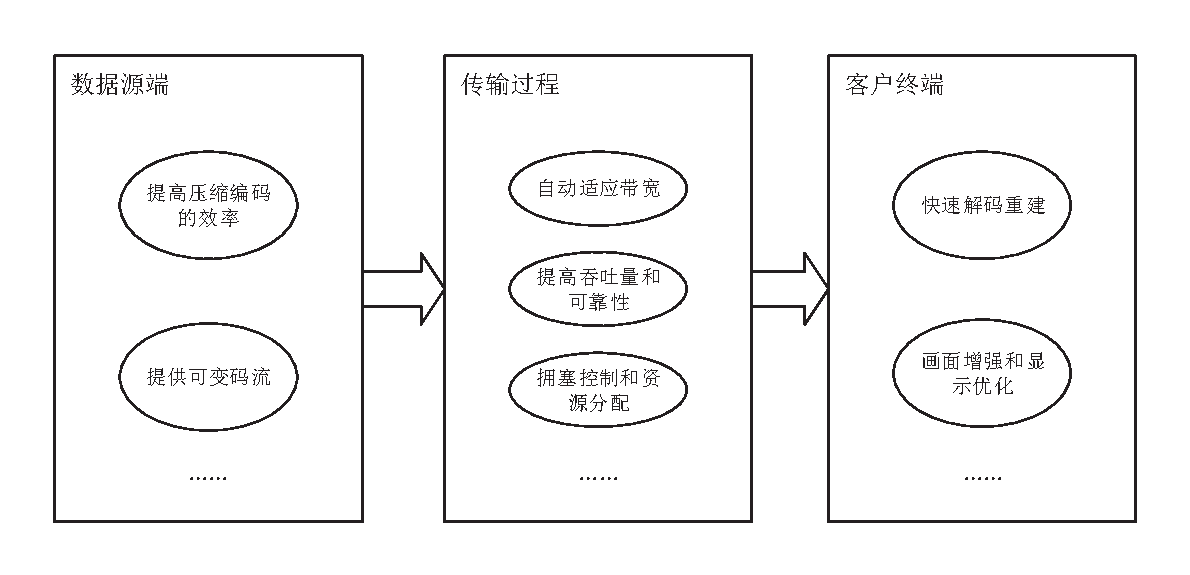
\includegraphics[width = 1.0\linewidth]{eps/research-framework}
	\caption{视频流媒体研究框架 \label{fig:research-framework}}
\end{figure}

数据源端对视频码流可变性的支持,再加上传输中自动调整码率以适应带宽的变化,结果就是所谓的自适应视频流媒体。在自适应视频流媒体中,服务器发送给客户端的视频流的码率能自动根据带宽的变化情况进行调整。这一特性能够很好地应对上一节中提到的网络异构和带宽波动带来的挑战。虽然其他方面的研究,例如对编码效率的提升、对网络架构和协议的改进,也非常重要,但本文主要关注的是自适应视频流媒体相关技术的研究。

通常有两种选择可以用来实现自适应视频流媒体。第一种选择是采取多码流的方法。多码流方法的原理很简单,就是预先编好不同码率的多个码流存放在服务器上,根据网络情况选取其中合适的一个进行传送。近年来兴起的HTTP动态自适应流媒体(Dynamic Adaptive Streaming over HTTP,  DASH)\supercite{Sodagar2011}就属于这类方法。如图\ref{fig:DASH}所示,DASH系统在服务器端提供不同码率的多个码流切片,客户端通过HTTP协议拉取数据,在某个时间段内可以选择性地接收这几个码流中任何一个的切片,通过在多码流之间切换来动态适应带宽波动。第二种选择是采用可伸缩视频编码\supercite{SVC-Overview}技术。作为国际视频编码H.264/AVC\supercite{H.264}的扩展之一,可伸缩视频编码目的就是在单个码流中加入伸缩性的支持,使其码率能够根据需要改变。因此,用它来实现自适应视频流媒体系统正符合其设计初衷。

\begin{figure}[t]
	\centering
	\includegraphics[width = 1.0\linewidth]{eps/DASH}
	\caption{DASH系统的工作原理示意图\label{fig:DASH}}
\end{figure}

多码流联播方案的优点是无需对已有的程序和系统做较大的改动,因此比较易于部署\supercite{Bouten2014}。很多商业视频网站(如YouTube、优酷等)已经用它实现了自适应功能。但是,多码流方案能提供的适应范围和粒度非常有限。例如,YouTube最多只提供240p、360p、480p、720p和1080p这五个等级,而优酷只提供标清、高清、超清这三个画质(参见图\ref{fig:13})。此外,多个码流的编码和存储需要大量的计算资源和磁盘空间,使得时间和空间开销成倍增加。要想以合理的代价提供精细无缝的自适应性,就需要采用可伸缩视频编码的方案。可伸缩视频码流能够以非常小的数据粒度进行码率调整,而且性能分析表明可伸缩视频编码的压缩效率远高于同一内容多次编码的多码流方法\supercite{SVC-Performance}。正是因为这些优势,采用可伸缩视频编码来实现自适应视频流媒体从技术上来说是一个更好的方案,也吸引了学术界很多研究者的关注\supercite{Chuah2012, Zhu2013, Dan2013, Yang2014, Cicalo2014}。

\begin{figure}[t]
	\centering
	\includegraphics[width = 1.0\linewidth]{clip/13.png}
	\caption{优酷网视频码率自适应功能图示\label{fig:13}}
\end{figure}

从图\ref{fig:research-framework}所示的研究框架中可以看出,采用可伸缩视频编码或是采用DASH之类的多码流方案,其区别只在于数据源端提供灵活码流的方式不同。可伸缩视频作为数据源时,在给定码率下如何最优地从整个码流中截取出一个子流用于发送是需要研究的问题之一,DASH系统则不存在这个问题。而对于在传输中如何自动调整码率以适应带宽的变化,却是二者共有的问题。此外,无论是何种视频流媒体系统,当用户设备收到视频流后都需要进行解码和播放。为了在计算资源有限的设备上满足实时播放的要求,通用处理器上的解码优化也是值得重视的问题之一。这些问题的解决,是提高视频流媒体服务质量和用户体验的关键。

\section{本文研究内容和主要贡献}

本文结合视频流媒体所面临的挑战,对上面提到的关键问题进行研究。首先,本文针对可伸缩视频数据源提出了新的失真模型和码流截取方案,在支持可变码率的同时提供尽可能高的视频质量;其次,本文为视频数据的传输过程设计了新的码率自动调整策略,用控制论的方法来解决适应带宽变化的问题;最后,为了保证用户终端收到码流后能够快速实时的解码并播放,本文研究了新一代国际视频编码标准HEVC(High Efficiency Video Coding)\supercite{HEVC-Overview}的解码过程,提出了新的优化算法来对其进行加速。本文主要的创新性贡献可以归纳为如下三个部分:
\begin{enumerate}
\item {采用线性误差模型的码流截取方案}\\
作为码率适应带宽波动的前提条件,视频流媒体中的数据源需要能够灵活调整。可伸缩视频编码将数据划分为基本层和增强层,通过丢弃增强层的数据包来实现即时码率变化。从完整的可伸缩码流中丢弃部分数据得到一个子流的过程称为码流截取。本文以最小化特定截取码率限制下的视频失真为目标,首先提出了一个线性误差模型来估计丢弃任意数据包组合带来的失真变化,然后利用它设计了一个贪心型算法来根据每个数据包的码率和失真影响对其赋优先级,作为截取过程中丢包的顺序。相比于参考软件,这一码流截取方案能够以更低的复杂度取得更高的视频质量。
\item {基于PID控制思想的码率自适应算法}\\
自适应流媒体的另一个关键问题是传输过程中的码率调整策略,即在可用带宽不断变化的情况下,决定何时调整码率并确定调整到多少。本文基于经典的比例-积分-微分(Proportional-Integral-Derivative,PID)控制思想,提出了一个综合考虑带宽的历史状况、当前状态和未来趋势的码率自适应算法,既能充分利用带宽,传输较高的视频质量,又能减小带宽波动的影响,保证视频质量的平滑性。该算法在点播和直播的实际测试中都表现出了很好的性能,而且很容易扩展到各种自适应流媒体系统。
\item {高度优化的HEVC解码器设计与实现}\\
视频流媒体的最后一个阶段是码流在用户终端设备上的解码播放。为此,本文设计并实现了一个高度优化的HEVC软件解码器,将数据级和任务级并行方法相结合,显著提高了各个解码模块的计算效率以及整体解码速度。该解码器分别在主流的桌面和移动处理器上达到了4K ($3840 \times 2160$) 和720p ($1280 \times 720$) 视频的实时解码要求,并已成功应用于业界知名的视频流媒体平台迅雷看看,为进一步改善用户在线观看视频的体验提供了技术支撑。
\end{enumerate}

\section{本文的结构安排}

本文共分为六章,后续章节具体内容安排如下。

第二章概述视频流媒体领域的研究基础和相关工作。首先对视频编码和流式传输的基础知识进行简要介绍,为后文内容做准备;然后结合本文的研究内容对码流截取、码率自适应、解码器优化这几个问题和已有工作进行分析。

第三章讨论采用线性误差模型的码流截取方案。首先针对可伸缩视频推导并验证线性误差模型,然后介绍采用该模型的失真估计方法和以码率失真影响为度量标准的优先级赋值算法。最后展现并分析所提出的码流截取方案的实验结果。

第四章讨论基于PID控制思想的码率自适应算法。首先对PID控制器做简单的介绍,然后将PID模型运用到视频传输中的码率自适应问题,提出了一个新颖的码率自适应算法。该算法被集成在了实际点播和直播流媒体系统中,其有效性通过对比实验得到了验证。

第五章讨论针对新一代视频编码标准HEVC的解码优化工作。以重新设计的解码器原型为基础,首先采用单指令多数据技术对特定解码模块进行加速,然后引入帧级并行解码框架提高了在多核处理器上进行多线程解码的速度,最后对上述方法所取得的优化效果进行了评测。

第六章总结全文内容并对未来工作和应用前景进行展望。
	\chapter{研究现状和相关工作}
本章介绍研究现状和相关工作。

\section{流媒体研究领域综述}

\section{视频编解码相关工作}

\section{SVC码流截取的相关工作}

\section{码率自适应的相关工作}
	\chapter{基于线性误差模型的码流截取}
本章介绍码流截取算法。

\section{问题描述}

\section{线性误差模型}

\subsection{模型推导}

\subsection{误差向量获取}

\subsection{模型验证}

\section{数据包优先级赋值}

\subsection{优先级度量标准}

\subsection{贪心法赋值}

\subsection{无参考源的情况}

\section{实验结果}

	\chapter{基于PID控制器的码率自适应算法}

\section{引言}

在实际网络条件下,带宽波动是不可避免的。对于一个视频流媒体系统而言,能够根据带宽变化来自适应地调整发送码率能为用户提供更好的服务。在上一章中,我们通过可伸缩视频的码流截取,使得码率能够调整;在本章中,我们主要关注如何调整。由于视频码率与视频质量一般来说是正相关的,调整码率也就是调整所传送视频的质量。因此,本章解决的问题又被称为质量控制问题。我们将基于经典控制实践中的PID思想,设计一个综合考虑带宽的历史状况、当前状态和未来趋势的码率自适应算法,从而提高发送视频的总体质量和平滑性。

\section{PID控制器简介}

PID控制器\footnote{http://en.wikipedia.org/wiki/PID\_controller}是一个在工业控制系统中常用的闭环反馈控制器。PID控制中的两个重要概念是过程变量和控制目标。过程变量代表着系统当前的状态,而控制目标是系统希望达到的理想状态。PID控制的基本思想就是根据过程变量和控制目标之间的误差来确定一个控制输出,该输出反馈作用到系统以最小化上述误差。

PID控制器的控制输出一般如下定义:
\begin{equation}
\label{eq:pid-output}
u(t) = {K_p} \cdot e(t) + {K_i} \cdot \int_0^t {e(\tau )d\tau }  + {K_d} \cdot \frac{d}{{dt}}e(t) \: ,
\end{equation}
其中$e(t)$指代过程变量与控制目标在时刻$t$的误差,$K_p$、$K_i$、$K_d$是三个可调参数,依次称为比例增益、积分增益和微分增益。公式(\ref{eq:pid-output})的结果通过某种方式来影响系统状态,使得过程变量朝着控制目标变化。

作为一个灵活有效的控制技术,PID可以被用来解决各种各样的控制问题\supercite{Wong2004}\supercite{Li1999}。在本文的工作中,我们基于它设计了一个码率自适应算法,用来控制视频流媒体中的视频质量。

\section{基于PID的码率自适应}

本节首先介绍质量等级的概念,来将视频流媒体中的视频质量和码率值离散化,接着定义在所提出的码率自适应算法中用到的过程变量及其控制目标。之后,我们详细解释控制模型和自适应算法细节,并简要讨论一下模型参数的选取和调优。

\subsection{质量等级划分}

视频质量或码率是一个连续的值,以任意的精度来控制或调整它是不现实的。因此,我们首先提出一个质量层级的概念来离散化视频质量和码率。当需要调整时,我们只是增加或减少质量等级。每一个质量等级对应一个确定的码率。高等级对应高码率,反之亦然。有多少个质量等级以及它们跟具体码率值如何对应可以根据实际需求来确定。质量等级越多,系统就能越精细地调整码率来适应带宽变化。如绪论中所说,用多码流实现的自适应流媒体系统只能提供有限的几个质量等级,而基于可伸缩视频编码的流媒体系统能够以更高的精度来定义质量等级。

\subsection{过程变量和控制目标}

在本文所提出的质量控制算法中,所选取的过程变量称为“实际与检测间隔比”。下面介绍其具体定义。

\begin{figure}[h]
	\centering
	\includegraphics[width = 0.9\linewidth]{figures/Intervals.png}
	\caption{达尔文流媒体服务器中的两个时间线 \label{fig:intervals}}
\end{figure}

在达尔文流媒体服务器中,有两个时间线非常重要。第一个是推送时间线(push time),也就是视频数据包被推送到缓冲区的时间;第二个是播放时间线(play time),也就是数据包应该在播放中被显示的时间(通常记作该数据包的PTS)。这两个时间线的关系如图\ref{fig:intervals}所示。服务器程序会定时检测这两个时间线,并根据数据包的延迟来决定是否需要调整发送的视频质量。图\ref{fig:intervals}中的两个间隔,即检测间隔(check interval)和实际间隔(actual interval),值得我们注意。在理想情况下,每次检测间隔中服务器推送的数据量应该恰好能实际播放等于检测间隔的一段时间,也就是\textit{actual\_interval} = \textit{check\_interval}。如果实际间隔小于检测间隔,说明这段时间内推送了较少的数据,推送数据变慢很可能是带宽有所下降。反过来,如果实际间隔大于检测间隔,说明这段时间内推送了较多的数据,意味着网络条件良好且数据被快速推向客户端。这两个间隔的比值,也就是所谓的“实际与检测间隔比”,能够反映当前推送的速率是否与网络带宽相符。

“实际与检测间隔比”适合用作质量控制有三方面的原因。第一,这个比例直接对应着适合带宽的码率与当前传输的码率的比值,只需据此进行调整就可以准确地使码率符合带宽。第二,根据定义这个比例的理想值就是1,这就是算法的控制目标,无需再通过别的方法确定。第三,这个值在实际系统中便于计算,普适性较好。

\subsection{控制模型}

在通常的PID控制器中,控制输出是用过程变量与控制目标之间的差值进行比例、积分、微分求取出来的。考虑到我们所选的过程变量是一个比例,且控制目标是1,本文对通常的PID控制器做了修改,提出了一个基于比例的模型。在这个模型中,过程变量直接被用来计算控制器输出,而且所有求差的运算都被适当的改为了求比例的运算,以保持模型的合理正确性,如下所示:

\begin{equation}
\label{eq:ut}
{u_t} = {K_p} \cdot E_p^t + {K_i} \cdot E_i^t + {K_d} \cdot E_d^t ,
\end{equation}

\begin{equation}
\label{eq:ep}
E_p^t = \frac{{actual\_interva{l_t}}}{{check\_interva{l_t}}} ,
\end{equation}

\begin{equation}
\label{eq:ei}
E_i^t = \frac{{long\_actual\_interva{l_t}}}{{long\_check\_interva{l_t}}} ,
\end{equation}

\begin{equation}
\label{eq:ed}
E_d^t = E_p^t/E_p^{t - 1} ,
\end{equation}

\begin{equation}
\label{eq:long-actual}
long\_actual\_interva{l_t} = \sum\limits_{\tau = {T_l}}^t {actual\_interva{l_\tau}} ,
\end{equation}

\begin{equation}
\label{eq:long-check}
long\_check\_interva{l_t} = \sum\limits_{\tau = {T_l}}^t {check\_interva{l_\tau}} .
\end{equation}

在公式(\ref{eq:ut})中:$K_p$、$K_i$、$K_d$分别表示比例部分、积分部分、微分部分的可调参数;$E_p^t$、$E_i^t$、$E_d^t$则对应各部分在第t次检测时的值,它们的定义如公式(\ref{eq:ep})至(\ref{eq:long-check})所示;控制器输出$u_t$将用来计算适合当前带宽的码率,并据此选择要传送的质量等级。

在公式(\ref{eq:long-actual})和(\ref{eq:long-check})中,$T_l$代表上一次质量等级改变的时间。按照理论定义,积分部分应该从系统启动开始记录,但在实际环境中,网络带宽有可能变动非常大,如果积分部分记录累积太长时间将不适合反映当前的网络条件,从而减缓调整质量的决策。因此这里采用了一个折衷,选择从上一次质量等级变化的时间开始计算积分部分。

这个基于比例的模型对于所选的过程变量和控制目标比通用模型更加简单有效。而且,在该模型中,当三个参数进行归一化处理后,控制器输出具备明显直观的意义。从公式(\ref{eq:ep})至(\ref{eq:long-check})容易看出,$E_p^t$、$E_i^t$、$E_d^t$这三个值都是在1附近波动的比值;而根据公式(\ref{eq:ut}),控制器输出$u_t$可以被视作这三个比值的加权平均(三个参数作为权值)。因此,$u_t$也是一个在1附近的比值,它对应着适合当前带宽的码率与当前发送码率的关系。换句话说,如果$u_t$大于1,那么控制器决定当前发送码率需要增加;反之,如果$u_t$小于1,意味着控制器认为当前发送码率需要减小。用$u_t$作为一个乘子来调整当前发送的码率,我们就能控制流媒体系统符合带宽的变化。

\subsection{自适应算法}

综上,本文提出的码率自适应算法描述如下:

\begin{algorithm}
	\caption{基于PID的码率自适应算法}
	\label{algo:control}
	\begin{algorithmic}
		\STATE 准备发送数据包
		\STATE check\_interval = curr\_time -- last\_check\_time
		\STATE actual\_interval = curr\_media\_time -- last\_check\_media\_time
		\STATE long\_check\_interval += check\_interval
		\STATE long\_actual\_interval += actual\_interval
		\STATE 根据公式(\ref{eq:ep}) - (\ref{eq:ed})计算$E_p^t$、$E_i^t$、$E_d^t$的值
		\STATE output = ${K_p} \cdot E_p^t + {K_i} \cdot E_i^t + {K_d} \cdot E_d^t$
		\STATE new\_bitrate = output * curr\_bitrate
		\STATE new\_level = get\_level(new\_bitrate, bitrate\_of\_level[])
		\IF {质量等级变化}
		\STATE long\_check\_interval = 0
		\STATE long\_actual\_interval = 0
		\STATE curr\_bitrate = bitrate\_of\_level[new\_level]
		\ENDIF
		\STATE 根据新的质量等级发送数据包
	\end{algorithmic}
\end{algorithm}

相比于其他的调度策略,这个基于PID的自适应算法具有以下几个优点。首先,该算法不仅仅依据当前状态或者固定时间点的信息来做决策,因此质量调整可以在任何合适的时间发生。其次,因为PID模型(微分部分)在某种程度上考虑了对未来的预测,该算法能够判断带宽在未来一段时间内是否会变得足够大或足够小,因此能避免一些不必要的调整。最后,该算法并不一定一次只调整一个质量等级,这就使得当带宽剧烈下降时能够快速下调质量以保证流畅播放,而当系统启动时能够快速上调质量以使用户尽早收到更清晰的视频。

\subsection{参数选取与调优}

与工业界的其他PID控制系统一样,本文提出的算法中三个参数的选取也是跟实现相关的。大多数情况下,为取得最优的效果,需要手动试错调节。每个参数对系统的不同方面产生影响,知道这些影响有助于进行参数选取。一般来说,PID控制器中的比例部分会影响系统的稳定性。如果比例增益$K_p$过高,系统容易变得不稳定。但是,太低的$K_p$又会导致过长的上升时间,使系统响应迟缓。积分部分除了能消除稳态误差,还能加速过程变量向控制目标的变化。这意味着,增大$K_i$能减小上升时间,提高系统的响应速度。但是,积分部分会累积过去一段时间的误差,使过程变量容易超出目标值(即超调),因此过大的$K_i$也会导致系统不稳定。上述这些隐患都能通过微分部分来校正。微分部分通过预测系统行为,具有减小超调、提高稳定性的双重效果。但是微分部分的特点是对误差分成敏感,也正是因为此,工业实践中微分增益$K_d$通常都设置的比较低。

本文采用了经典的Ziegler--Nichols方法\supercite{Ziegler1942}来进行参数选取。该方法首先把积分和微分参数设为0,调节比例参数$K_p$到系统开始震荡时的值$K_u$,假设震荡周期为$T_u$,那么设置$K_p = 0.6K_u$、$K_i = 2K_u/T_u$、$K_d = K_u \cdot T_u/8$。再将$K_p$、$K_i$和$K_d$进行归一化,就得到最终的参数:$K_p = 0.22$,$K_i = 0.73$,$K_d = 0.05$。

\section{实验结果}

\section{本章小结}
	\chapter{高度优化的HEVC解码器}

新的视频编码标准HEVC虽然显著提高了编码效率,但其复杂度也有了明显的提升。现有的用户设备计算资源有限,如何快速实时的解码成为了HEVC广泛应用于流媒体系统的一个阻碍。在硬件解码芯片普及之前,软件解码器的实现和优化是一项重要且有挑战性的工作。在本章中,我们给出了一个高度优化的HEVC软件解码器,并对其在不同处理器平台上的速度进行了测试。

\section{新的解码器原型设计}

HEVC标准化组织提供的参考软件HM中虽然包含了一个HEVC解码器的实现,但是这个实现主要目的是为了方便标准制定和相关的研究性实验,其结构冗余复杂,解码效率低下,不适合实际使用。为了确保本文后续优化工作的有效性和实用性,我们自行设计了一个新的解码器原型。

\begin{figure}[t]
	\centering
	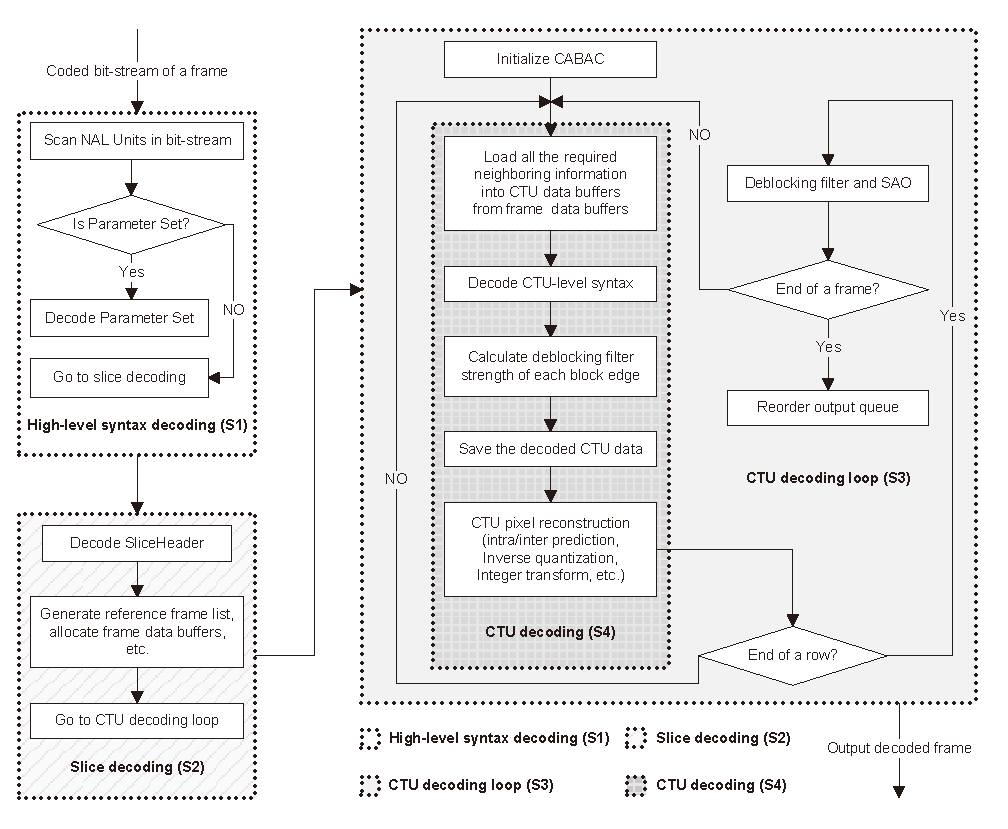
\includegraphics[width = 1.0\linewidth]{eps/decoding_workflow}
	\caption{\label{fig:decoding_workflow}新的解码器原型流程框架}
\end{figure}

该解码器原型的四阶段流程框架如图\ref{fig:decoding_workflow}所示,其中列出了解码器结构中的四个关键阶段,即:高层语法解码、slice解码、CTU\footnote{Coding Tree Unit,HEVC中的基本解码单元,类似H.264/AVC中的宏块}解码循环和CTU解码,对应图中的S1-S4。这个解码器原型有两个不同于HM中参考解码器的特性。第一,在CTU解码(S4)的开始阶段,数据会从全局性的帧缓冲区拷贝一份到CTU缓冲区。这样可以保持这个CTU解码过程中数据访问的局部性,从而降低处理器的缓存失效率。该特性有助于接下来要讨论的单指令多数据(SIMD)优化算法。第二,在CTU解码循环(S3)中,去块滤波和SAO这些理论上要等整帧解完之后才进行的操作,会在每个CTU的像素重建之后立即开始。这样使得这个CTU能够尽早被参考,也就意味着更多的解码任务可以并行执行。该特性为本文后面要介绍的帧级多线程解码框架打下了基础。

需要指出的是,虽然第一个特性有助于提高缓存命中率,但增加了数据拷贝的额外开销。为了尽量减小这一开销,我们会严格选择所需数据:对于当前的CTU解码,只有它上面和左边的CTU可能被用到;而且这两个CTU中有用的分别只是下边界和右边界的数据。按需进行精细复制可以避免大量多余的内存拷贝操作。另外的内存优化还包括对帧缓冲区的处理。所有帧缓冲区都被设计为全局的,只在解码程序开始时统一分配,解码过程中以内存池的方式进行管理,程序运行结束后统一释放。这一机制尽量避免了频繁地内存分配和释放操作,有利于提高程序的内存使用效率和执行速度。

在这一全新的解码器原型基础上,我们接下来用SIMD优化和多线程并行这两种方法来对整个解码过程进行加速。

\section{耗时模块的加速}

大多数现代通用处理器都有SIMD扩展指令集,例如x86架构上的MMX、3DNow!、SSEx、AVX等\supercite{Intel-manual},以及ARM架构上的NEON\supercite{ARM-manual}。这类指令集中的一条指令可以同时操作位于特殊向量寄存器中的多个数据,能成倍地提高数据吞吐率。在这一节中,我们用SIMD技术来加速HEVC解码中的几个耗时模块。

\begin{table}
	\begin{center}
		\caption{HEVC解码过程中各个模块的时间占比} \label{table:HEVC_timing}
		\renewcommand{\arraystretch}{1.5}
		\begin{tabular}{c|c}
			\hline
			\textbf{解码模块} & \textbf{时间占比} \\
			\hline
			\hline
			运动校正 & $47.88\%$ \\
			\hline
			反变换 & $14.5\%$ \\
			\hline
			熵解码 & $12\%$ \\
			\hline
			去块滤波 & $7.76\%$ \\
			\hline
			采样自适应偏移 & $5.12\%$ \\
			\hline
			内存操作 & $5\%$ \\
			\hline
			反量化 & $2.24\%$ \\
			\hline
			其他 & $5.5\%$ \\
			\hline
		\end{tabular}
	\end{center}
\end{table}

根据对HEVC解码过程时间分布的测量统计\supercite{Duan2014},较高码率的码流在解码中各个模块的时间消耗比例如表\ref{table:HEVC_timing}所示。其中耗时较多且适合用SIMD来优化的几个模块包括:运动校正、反变换、去块滤波和采样自适应偏移(熵解码虽然耗时较多,但不适合用SIMD技术进行优化;而且据我们所知没有很好的加速方法)。这几个模块中,运动校正和反变换已经在Yan等人的工作\supercite{Yan-VCIP2012}中被充分地优化过了,本文直接采用其中的结果并对部分操作进行了改进;而对于已有工作尚未很好处理的去块滤波和采样自适应偏移,我们将分别设计全新的算法对其进行加速。下面介绍的算法对x86架构和ARM架构都适用,在具体实现上有差异的地方我们会单独指出。

\subsection{低复杂度运动校正算法}

在HEVC中,运动校正的实质是水平方向和竖直方向的插值。每个方向的插值都是用8抽头的DCT插值滤波器来求取亮度分量的目标值,用4抽头的DCT插值滤波器来求取色度分量的目标值。求值公式分别为:
\begin{equation}
\label{equ:formula-DCT-IF-1}
Component_{luma} = \sum_{m=0}^7 p_m \times L_m
\end{equation}
和
\begin{equation}
\label{equ:formula-DCT-IF-2}
\quad Component_{chroma} = \sum_{m=0}^3 q_m \times C_m,
\end{equation}
其中$L_0$ ~ $L_7$和$C_0$ ~ $C_3$分别表示亮度分量和色度分量的原始值,而$p_0$ ~ $p_7$和$q_0$ ~ $q_3$表示相应的插值系数组(group of interpolation coefficients,简称GIC)。亮度分量和色度分量运动补偿的精度分别是$1/4$像素和$1/8$像素;这意味着,在水平和竖直两个方向上,亮度分量都有4个待插值的位置,色度分量都有8个待插值的位置。图\ref{fig:luma_position}和图\ref{fig:chroma_position}分别展示了亮度和色度在水平方向的待插值位置。表\ref{table:coeff_position}对应列出了求取各个位置目标值的插值系数组。由该表和公式(\ref{equ:formula-DCT-IF-1})可以知道,如果得到一个亮度位置的目标值在水平方向和竖直方向都需要插值,那么这个求取过程将需要多达72次乘法运算。这就是运动校正主要的耗时因素。

\begin{figure}[!tp]
	\centering
	\includegraphics[width = 0.95\linewidth]{eps/luma_position}
	\caption{\label{fig:luma_position}
		HEVC运动校正亮度分量水平插值采用的8抽头DCT插值滤波器}
	% \vspace{5pt}
\end{figure}

\begin{figure}[!tp]
	\centering
	\includegraphics[width = 0.95\linewidth]{eps/chroma_position}
	\caption{\label{fig:chroma_position}
		HEVC运动校正色度分量水平插值采用的4抽头DCT插值滤波器}
	% \vspace{5pt}
\end{figure}

\begin{table}[!tp]
	\begin{center}
		\caption{HEVC运动校正中的插值系数组} \label{table:coeff_position}
		\renewcommand{\arraystretch}{1.3}
		\begin{tabular}{c|p{1cm}|p{1cm}|p{1cm}|p{1cm}|p{1cm}|p{1cm}|p{1cm}|p{1cm}}
			\hline
			\textbf{亮度分量位置} & \textbf{$p_0$} & \textbf{$p_1$} & \textbf{$p_2$} & \textbf{$p_3$} & \textbf{$p_4$} & \textbf{$p_5$} & \textbf{$p_6$} & \textbf{$p_7$} \\
			\hline
			\hline
			$L_3$ & $0$ & $0$ & $0$ & $64$ & $0$ & $0$ & $0$ & $0$ \\
			\hline
			$a$ & $-1$ & $4$ & $-10$ & $58$ & $17$ & $-5$ & $1$ & $0$ \\
			\hline
			$b$ & $-1$ & $4$ & $-11$ & $40$ & $40$ & $-11$ & $4$ & $-1$ \\
			\hline
			$c$ & $0$ & $1$ & $-5$ & $17$ & $58$ & $-10$ & $4$ & $-1$ \\
			\hline
			\hline
			\textbf{色度分量位置} & \multicolumn{2}{|c|}{\textbf{$q_0$}} & \multicolumn{2}{c}{\textbf{$q_1$}} & \multicolumn{2}{|c|}{\textbf{$q_2$}} & \multicolumn{2}{c}{\textbf{$q_3$}} \\
			\hline
			\hline
			$C_1$ & \multicolumn{2}{|c|}{\textbf{$0$}} & \multicolumn{2}{c}{\textbf{$64$}} & \multicolumn{2}{|c|}{\textbf{$0$}} & \multicolumn{2}{c}{\textbf{$0$}} \\
			\hline
			$d$ & \multicolumn{2}{|c|}{\textbf{$-2$}} & \multicolumn{2}{c}{\textbf{$58$}} & \multicolumn{2}{|c|}{\textbf{$10$}} & \multicolumn{2}{c}{\textbf{$-2$}} \\
			\hline
			$e$ & \multicolumn{2}{|c|}{\textbf{$-4$}} & \multicolumn{2}{c}{\textbf{$54$}} & \multicolumn{2}{|c|}{\textbf{$16$}} & \multicolumn{2}{c}{\textbf{$-2$}} \\
			\hline
			$f$ & \multicolumn{2}{|c|}{\textbf{$-6$}} & \multicolumn{2}{c}{\textbf{$46$}} & \multicolumn{2}{|c|}{\textbf{$28$}} & \multicolumn{2}{c}{\textbf{$-4$}} \\
			\hline
			$g$ & \multicolumn{2}{|c|}{\textbf{$-4$}} & \multicolumn{2}{c}{\textbf{$36$}} & \multicolumn{2}{|c|}{\textbf{$36$}} & \multicolumn{2}{c}{\textbf{$-4$}} \\
			\hline
			$h$ & \multicolumn{2}{|c|}{\textbf{$-4$}} & \multicolumn{2}{c}{\textbf{$28$}} & \multicolumn{2}{|c|}{\textbf{$46$}} & \multicolumn{2}{c}{\textbf{$-6$}} \\
			\hline
			$i$ & \multicolumn{2}{|c|}{\textbf{$-2$}} & \multicolumn{2}{c}{\textbf{$16$}} & \multicolumn{2}{|c|}{\textbf{$54$}} & \multicolumn{2}{c}{\textbf{$-4$}} \\
			\hline
			$j$ & \multicolumn{2}{|c|}{\textbf{$-2$}} & \multicolumn{2}{c}{\textbf{$10$}} & \multicolumn{2}{|c|}{\textbf{$58$}} & \multicolumn{2}{c}{\textbf{$-2$}} \\
			\hline
		\end{tabular}
	\end{center}
\end{table}

DCT插值滤波是一个典型的向量乘法过程。本文对于水平和竖直方向的插值滤波分别设计了最优的SIMD算法来提高计算效率。对于水平方向的DCT插值滤波,我们采取了已有工作\supercite{Yan-VCIP2012}中的算法,因为其充分利用了寄存器,能够同时对8个亮度分量进行插值。如图\ref{fig:DCT-IF_luma}所示,该算法的流程如下。首先插值系数组$p_0$ ~ $p_7$被重复装入向量寄存器$R_0$,然后原始像素$L_0$ ~ $L_{14}$被装入向量寄存器$R_1$。然后,为了尽可能充分地利用向量寄存器,$R_1$中的15个像素值被逐次交织装入向量寄存器$R_2$ ~ $R_5$。最后如图所示通过4条PMADDUBSW指令和3条PHADDW指令,就可以在寄存器$R_2$中得到8个插值后的16比特亮度分量,这些值通过一条MOVDQA指令就能存回到内存中去。平均下来,水平方向上每个亮度分量的DCT插值滤波只需要$1/2$条PSHUFB指令、$1/2$条PMADDUBSW指令、$3/8$条PHDDW指令以及个$1/8$条存取指令,有效节省了计算时间。

\begin{figure}[!tp]
	\centering
	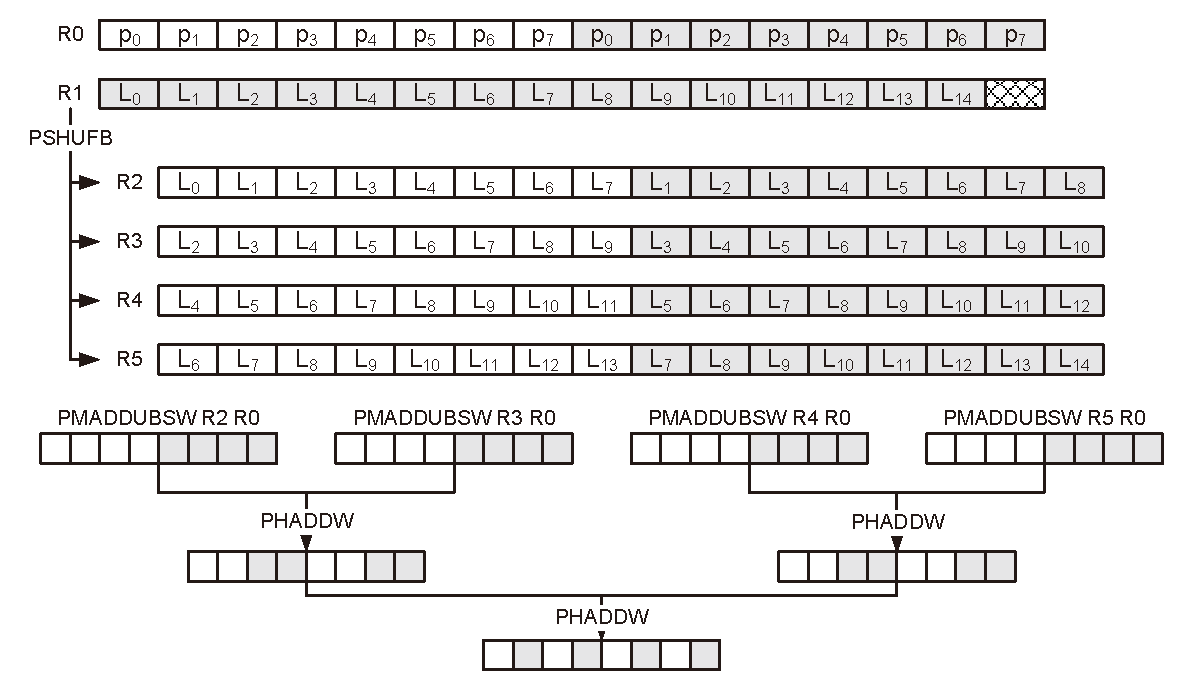
\includegraphics[width = 0.95\linewidth]{eps/DCT-IF_luma}
	\caption{\label{fig:DCT-IF_luma}
		低复杂度运动校正的水平插值图示}
	% \vspace{5pt}
\end{figure}

对于竖直方向的DCT插值滤波,使用PMADDUBSW指令不再可行。之前的工作普遍采用了重复进行乘法与加法的方法。这样的话得到一个插值后的亮度分量平均需要$1$条乘法指令与$7/8$条加法指令。这里我们提出一个无乘法的竖直方向DCT插值滤波算法,以进一步减少所需指令数目,并对16个亮度分量进行并行插值。该算法的基本思想是提取出向量乘法中的公共计算部分,并尽可能多地重用它们。目的是用低复杂度的加减法运算和移位运算的组合来取代乘法运算。例如,在位置$a$和位置$b$的亮度分量目标值可以用以下重新组织的计算方式求得:
\begin{eqnarray}
component_{luma,a} &=& T_0 + ((T_0+L_1)<<2) + (L_3<<5)
\nonumber 
\\&& + L_4 + ((L_3+L_4)<<4)- L_0 + L_6,
\end{eqnarray}
和
\begin{eqnarray}
component_{luma,b} &=& ((L_1+L_6)<<2) - (L_0+L_7)
\nonumber 
\\&& - T_1 + T_2 + (T_2<<2),
\end{eqnarray}
其中:
\begin{equation}
T_0 = ((L_3 - L_2)<<1),
\end{equation}
\begin{equation}
T_1 = L_2 + L_5,
\end{equation}
\begin{equation}
T_2 = ((L_2 + L_5)<<3) - (T_1<<1).
\end{equation}
这些就是所谓的公共计算部分。类似地,位置$d$、$e$、$f$和$g$的色度分量目标值可分别被重新组织为:
\begin{eqnarray}
component_{chroma,d} &=& (C_1<<4) + (C_1<<5) + (T_3<<3)
\nonumber 
\\&& + ((T_3 - C_0 - C_3)<<1),
\end{eqnarray}
\begin{eqnarray}
component_{chroma,e} &=& (C_1<<5) + ((C_1+C_2)<<4) 
\nonumber 
\\&& + ((C_1-C_0)<<2) + ((C_1-C_3)<<1),
\end{eqnarray}
\begin{eqnarray}
component_{chroma,f} &=& (C_1<<3) + ((C_1+C_2)<<5) 
\nonumber 
\\&& + (T_1<<4) + ((T_4-C_2-C_3)<<2),
\end{eqnarray}
和
\begin{equation}
component_{chroma,g} = (T_3<<5) + ((T_3-C_0-C_3)<<2), 
\end{equation}
其中$T_3 = C_1 + C_2$和$T_4 = C_1 - C_0$为公共计算部分。对于位置$c$和$h$、$i$、$j$,其公共计算部分的推导过程分别与位置$a$和$f$、$e$、$d$是对称的,此处不再重复说明。对于位置$L_1$和$C_1$,所需的乘法操作直接用移位运算代替即可。采用上述无乘法的算法,求取位置$a$或$c$的亮度分量目标值平均只需$1/2$次移位、$3/8$次减法以及$7/8$次加法运算,而对于位置$b$则只需$1/2$次移位、$3/8$次减法以及$3/4$次加法运算。相比之前工作中的SIMD算法,本算法的指令数目和复杂度均有所降低。类似的方法和结论也适用于色度分量的插值。

综上,运动校正模块通过SIMD算法能够减少所需指令数目、降低指令复杂度,从而提高执行速度,为整个HEVC解码过程节省可观的时间。

\subsection{无转置整数变换算法}

在HEVC中,整数变换及其反变换的实质仍然是矩阵乘法,可表示为如下形式:
\begin{equation}
R = T^TXT,
\end{equation}
其中$T$是变换矩阵,$X$是经过反量化之后的系数矩阵,$R$为结果矩阵。在通常的实现中,变换是通过先列变换再行变换的两阶段方式进行的:
\begin{equation}\label{equ:formula-transform-step1}
Step1:	\quad B_{i,j} = \sum_{k=0}^n A_{i,k}X_{k,j},
\end{equation}
以及
\begin{equation}\label{equ:formula-transform-step2}
Step2:	\quad R_{i,j} = \sum_{k=0}^n B_{i,k}A_{j,k},
\end{equation}
其中$B$为中间结果矩阵,$A = T^T$,表示变换矩阵的转置。根据公式(\ref{equ:formula-transform-step1})和(\ref{equ:formula-transform-step2}),虽然$A$可以预先装载,但在每一个列变换之前,$X$仍然需要先转置然后才能够有效装载进向量寄存器。这不仅带来了大量的数据访问开销,而且还占用了用于并行数据操作的向量寄存器,因此应该设法去除转置操作。

\begin{figure}[!t]
	\centering
	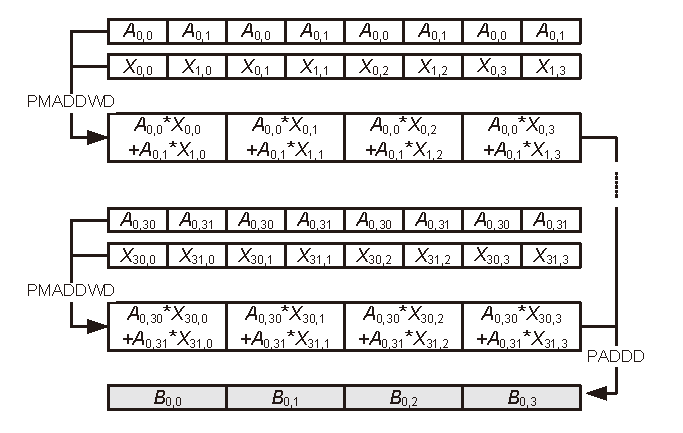
\includegraphics[width = 0.95\linewidth]{eps/transpose-free_IT}
	\caption{\label{fig:transpose-free_IT}
		无转置整数变换算法的核心过程}
	% \vspace{5pt}
\end{figure}

为了达到这个目标,本文提出了一种无转置的列变换算法。图\ref{fig:transpose-free_IT}展示了该算法的核心过程。图中显示了对于$32 \times 32$大小的变换单元的列变换,如何计算中间结果矩阵$B$的前四个系数。该算法的关键在于预装载之后的数据排布:当矩阵$A$一行中每两个元素重叠放入一个向量寄存器,且矩阵$X$的每两行元素交织放入另一个向量寄存器之后,这两个寄存器就可以进行向量乘法运算。对于$N \times N$ ($N = 8, 16, 32$) 的变换单元,使用$N/2$条PMADDWD指令和$N/2 - 1$条PADDD指令,可以得到中间结果矩阵$B$的4个元素。这些32比特的元素可以直接用于行变换,不再需要额外的存储或转置,从而有效地减少了指令数目并且保证了寄存器的高效利用。由于所有矩阵的缓冲区都是16-byte对齐的,变换中数据访问的开销也已降至最低。

读者可能会问这里能否用上一小节中针对运动校正设计的低复杂度算法来取代乘法操作。需要指出的是,在HEVC中,对不同大小的变换单元其变换矩阵是不同的,因此难以找到公共计算部分。在这种情况下对变换中的向量乘法进行拆分反而会增加指令数目并对性能产生不利影响。另外还要指出,向量寄存器资源的限制仍然是HEVC中变换过程SIMD算法的瓶颈。因为对于$16 \times 16$以及$32 \times 32$大小的变换单元,变换过程中各个矩阵的元素必须被分为多个部分并被多次装载,来分批完成整个变换过程。对此请参见本节末尾的讨论。

\subsection{对称去块滤波算法}

在HEVC的去块滤波中,对于8x8的块边界,每次以4个像素为单元来决定是否需要进行滤波,并决定是进行高强度滤波还是普通滤波。这样就把边界同一侧每次操作的像素个数限制为4,无法充分利用向量寄存器同时对8个像素进行计算。为了提高并行度,我们设计了一个与Yang等人在H.264/AVC解码器优化工作\supercite{Yang-TCE2006}中的描述类似的对称去块滤波算法。

\begin{figure}[h]
	\centering
	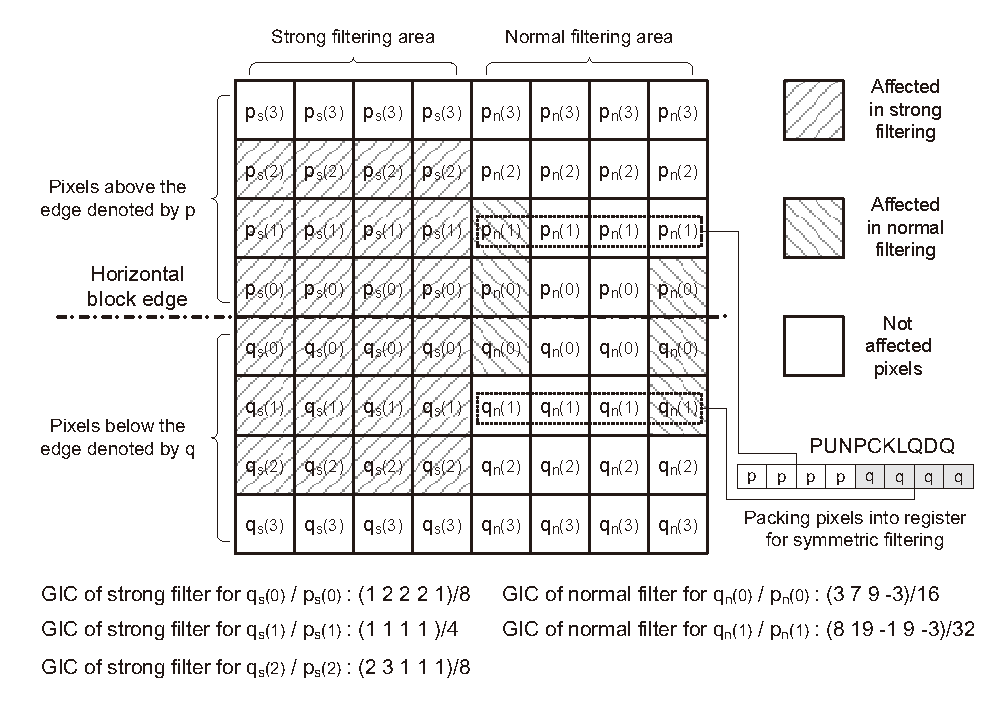
\includegraphics[width = 1.0\linewidth]{eps/vertical_DF_to_horizontal_edge}
	\caption{\label{fig:vertical_DF_to_horizontal_edge}HEVC中对$8 \times 8$块的水平边界进行滤波的操作示意图}
\end{figure}

图\ref{fig:vertical_DF_to_horizontal_edge}展示的是HEVC标准中对8x8块的水平边界进行滤波的操作示意图。滤波操作实质上就是对边界两侧的像素进行修改。在每侧的4个像素中,高强度滤波会修改其中的3个,普通滤波会修改其中的2个或1个或0个。修改的方法可以认为是一个插值的过程。原来的像素会被改为用它上下的像素进行插值(加权平均)的结果,从而实现像素值的平滑,达到消除边界的目的。在图\ref{fig:vertical_DF_to_horizontal_edge}所示的例子里,左边四列像素进行的是高强度滤波,右边四列是普通滤波。图的下方列出了对各个像素进行修改时用到的插值系数组,相当于滤波器的冲激响应\supercite{Norkin-TCSVT2012}。这里有一个比较关键的地方在于,根据HEVC对滤波模块的规定,边界两侧相同位置的像素,其GIC是一样的,而且插值所用的像素也是对称的。利用这个性质,我们可以用PUNPCKLQDQ这一SIMD指令把边界两侧相同位置的像素放在一个寄存器里同时参与计算。如图\ref{fig:vertical_DF_to_horizontal_edge}中所示,在高强度滤波中,对于0~3的每一个$i$,标记为$p_n(i)$的4个像素和标记为$q_n(i)$的4个像素放在一起;同样的,在普通滤波中,对于0~3的每一个$j$,标记为$p_s(j)$的4个像素和标记为$q_s(j)$的4个像素放在一起。这样,无论是哪种滤波方式,每次能处理8个像素,充分利用了128位向量寄存器(在滤波操作中因为要存储中间值,每个像素需占用16位),使得滤波操作所需的指令数减少了一半。

对于普通滤波方式来说,因为受影响的像素数不确定(0个到2个都有可能),所以在与高强度滤波同样的方式计算出滤波结果之后,还要另外用某种阈值来决定哪些像素最终会被滤波结果取代。这时可以用阈值来构造掩模,用掩模去选择最终结果。例如,对于图\ref{fig:vertical_DF_to_horizontal_edge}中的$q_n(0)$和$p_n(0)$行,中间两个像素不受影响,所以其4 x 16bit掩模应为:
\begin{equation}
Mask = \{ \texttt{0xffff}, \quad \texttt{0}, \quad \texttt{0}, \quad \texttt{0xffff} \}.
\end{equation}
基于此,普通滤波的最终结果可确定为:
\begin{equation}
ResultRow = (OriginalRow \land \neg Mask ) \lor (FilteredRow \land Mask).
\end{equation}
这些操作可以用并行逻辑运算指令PAND、PANDN以及POR很轻易地实现。

上面讨论的是水平边界的滤波。对于竖直边界,该算法过程是一致的,只需要先进行一次转置,然后按照上述方法进行计算即可。

\subsection{并行索引SAO算法}

在HEVC解码中,去块滤波之后的像素需要先进行采样自适应偏移(SAO)才能输出为解码图像。对于每个CTU,其像素进行SAO的模式由码流中解析出的\textit{SAOType}来指定。SAO模式有两种,一个是条带(Band)模式,一个是边缘(Edge)模式。这两种模式都会在原像素值上增加一个偏移量。不同之处在于,在条带模式中,这个偏移量由原像素值本身(0~255)来索引,而在边缘模式中,这个偏移量由原像素与其两个相邻像素的梯度值来索引。在条带模式中,每个条带横跨的像素值为4,因此256个不同像素值被分为了32个条带,作为索引去查表决定加到该像素上的偏移量。这样的索引操作在ARM架构上可以用NEON指令集扩展中的并行查表指令进行优化。然而遗憾的是,x86架构下没有对应的指令,只能用普通代码实现。相比于条带模式,边缘模式更为复杂,也是本节提出的并行索引SAO算法主要针对的一种模式。下面进行详细介绍。

\begin{figure}[t]
	\centering
	\includegraphics[width = 0.95\linewidth]{eps/SAO_edge_direction}
	\caption{\label{fig:SAO_edge_direction}HEVC中的SAO在边缘模式下选取相邻像素的4种方向}
\end{figure}

\begin{figure}[t]
	\centering
	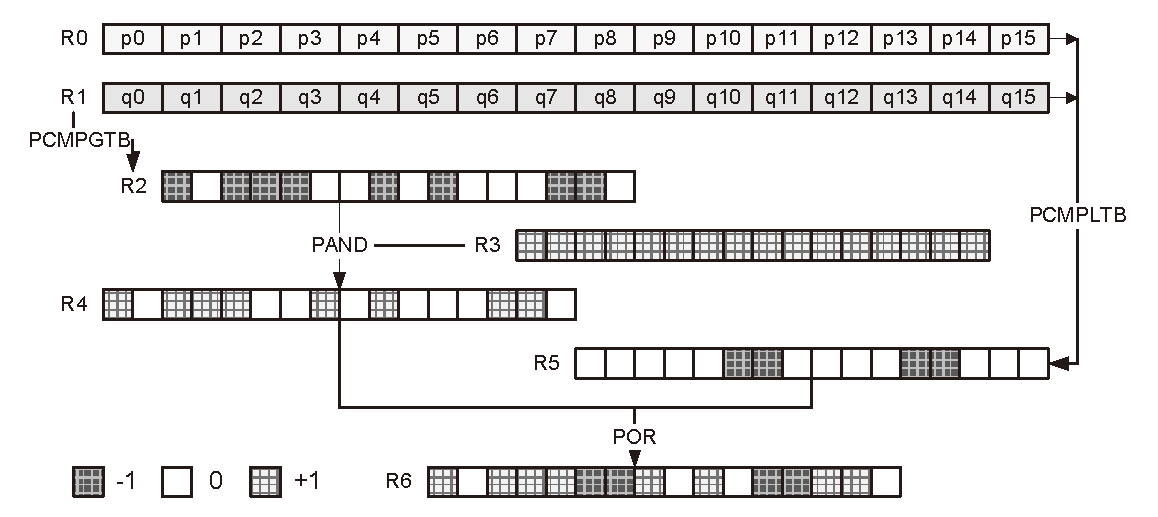
\includegraphics[width = 0.95\linewidth]{eps/SAO_edge_parallel_index}
	\caption{\label{fig:SAO_edge_parallel_index}HEVC中的SAO在边缘模式下的得到16个符号值的过程}
\end{figure}

在边缘模式中,一个像素要减去与它相邻的两个像素。这两个邻居所在的方向可以从图\ref{fig:SAO_edge_direction}中的四个方向选择其一。相减得到两个差值,差值根据其正负或0对应到1、-1和0这三个符号;将两个差值对应的符号相加(可能的结果为-2、-1、0、1、2),作为偏移量的索引。因为一个CTU中的所有像素相减方向都相同,所以计算索引的操作可以并行执行。对于128位的向量寄存器来说,一次可以处理16个像素。图\ref{fig:SAO_edge_parallel_index}展示了我们设计的并行索引算法的核心过程,其中用一对PCMPGTB/PCMPLTB指令和一对PAND/POR指令得到了16个像素相减的符号值。根据选定的方向求出两组符号值之后,通过PADDB指令将它们相加就得到16个索引值,最后用一条PSHUFB指令来查表得到所需的偏移量。很明显这种并行索引SAO算法已经取得了最大的数据级并行度,指令数量已经压缩到最少。需要指出的是,对于图\ref{fig:SAO_edge_direction}中$0^\circ$、$45^\circ$和$135^\circ$这三个方向的相减,将正确的像素取到向量寄存器中会有无法避免的开销,因为要访问的内存是非连续的。


需要指出的是,对于一些比较老的x86机器,其处理器只支持较早期版本的指令集扩展(如SSE2、SSE或MMX),因此上面优化中用到的一些高级指令(如PHADDW、PMADDUBSW等)可能无法使用。为了兼容性考虑,在检测到这样的机器时,一些横向的并行数据操作必须用所支持的较简单指令来实现,这时会有一定的速度牺牲。相反,对于某些支持AVX的最新处理器,向量寄存器的长度由128位扩展到了256位,数据吞吐率可以再提高一倍,这样就能进一步加速这些采用SIMD进行优化的模块。同理,在移动设备上ARM处理器提供的向量寄存器的个数更多,而且SIMD指令集更加智能(能很容易实现转置操作和条带模式SAO中的并行索引),这都能作为速度提升的空间。

总之,在我们所提出的解码器原型基础上,SIMD算法被用于优化大多数耗时解码模块,显著提高了其运行效率。在下一节中,我们将给出一个基于帧的并行解码框架,作为解码器优化的最后一步。

\section{帧级并行解码框架}

\begin{figure}[!t]
	\centering
	\includegraphics[width = 0.95\linewidth]{eps/parallel_decoding_framework}
	\caption{\label{fig:parallel_decoding_framework}HEVC帧级并行解码框架图}
\end{figure}

随着多核处理器的普及,并行算法成为了发挥这些处理器能力的必需。在本节中,我们提出了一个帧级的并行解码框架,可以在通过多线程取得几倍的解码加速比。该框架如图\ref{fig:parallel_decoding_framework}所示,其工作流程说明如下:
\begin{enumerate}
	\item 首先是解码器初始化;然后在收到码流数据时,入口线程(即主线程)调度第一个可用线程开始解码。
	\item 当第一个可用线程收到码流后,它立即完成slice解码(即图\ref{fig:decoding_workflow}中的S2阶段),并先向主线程发送解码上下文准备好的信号,然后才进入CTU解码循环(即图\ref{fig:decoding_workflow}中的S3阶段)。
	\item 主线程收到解码上下文准备好的信号后,它会把解码上下文信息拷贝到其他可用线程,并调度它们并行地开始后续帧的CTU解码循环。
\end{enumerate}

从该流程和图\ref{fig:parallel_decoding_framework}可以看出,所谓的并行任务指的是不同帧的CTU解码循环及CTU解码过程可以并发地执行,但高层语法和每一帧的slice解码阶段还是需要按照特定的顺序进行。

在本文提出的帧级并行解码框架中,帧内预测的帧是相对独立的,其解码过程与单线程一样。但对于帧间预测的帧,由于运动校正依赖于参考帧的重建像素,所以必须设立线程同步机制。为了平衡同步开销和并发任务的粒度,该框架使用了像素行级别的同步点。对每一帧,有一个变量用于指示该帧的哪一行已经完成解码重建。参考它的帧通过不断检查这一变量,就能在其所依赖的像素行准备好后立即开始进行运动校正。这样的设计用较小的开销解决了解码中的数据依赖问题,提高了潜在的并行度。

\section{优化结果}

在本节中,我们通过详尽的解码速度测试数据来展示整体优化结果。

对于x86架构平台,我们选用了Intel i7-2600 3.4GHz四核处理器,机器内存8GB,操作系统为Microsoft Windows 7。HEVC标准测试序列用HM 10编码器编码,重要的编码配置参见表\ref{table:HM_config}。

\begin{table}[t]
	\begin{center}
		\caption{生成测试码流所采用的HM编码配置} \label{table:HM_config}
		\renewcommand{\arraystretch}{1.5}
		\begin{tabular}{c|c}
			\hline
			\textbf{编码参数选项} & \textbf{参数值} \\
			\hline
			\hline
			Bit Depth & $8$ \\
			\hline
			CTU Size / Depth & $64$ / $4$ \\
			\hline
			IT Kernel size & $4 \times 4$ - $32 \times 32$ \\
			\hline
			Hadamad ME & Y \\
			\hline
			RDOQ & Y \\
			\hline
			SAO & Y \\
			\hline
			AMP & N \\
			\hline
			DF & Y \\
			\hline
			Temporal MVP & Y \\
			\hline
			Sign Bit Hiding & Y \\
			\hline
		\end{tabular}
	\end{center}
\end{table}

为了得到不同码率的码流,我们采用了四个QP值:23、28、33、38。对于每一个QP值和每一个测试序列,编出的码流分别用本文所实现的解码器、HM参考软件中的解码器、业界知名的多媒体框架FFmpeg\footnote{http://ffmpeg.org}中的解码器进行解码,比较三者的解码帧率。我们的解码器和HM都是用Microsoft Studio 2008编译得到,而FFmpeg是从网上下载的可执行文件\footnote{http://ffmpeg.zeranoe.com/builds/}。标准测试集中的A类(2560x1600)和B类(1920x1080)序列的测试结果参见表\ref{table:decoding_speed_x86}。表中的加速比都是相对于HM计算得到的结果。从中可以看出,在四线程解码时,我们的解码器相比于HM 10.0有平均13.21倍的速度提升,FFmpeg虽然也比HM 10高效得多,但其性能只有我们的三分之一不到。我们的解码器相对于FFmpeg的加速比在单线程和多线程下分别为6.13/2.18=2.81和13.21/3.59=3.68。帧级并行解码框架的有效性可以从多线程比单线程的加速比体现出来。我们的解码器4线程比单线程速度提高了2.15倍(13.21/6.13),而FFmpeg的4线程只比单线程速度提高了1.65倍(3.59/2.18)。

\begin{table}[t]
	\begin{center}
		\caption{x86平台的三种HEVC解码器的解码速度对比} \label{table:decoding_speed_x86}
		\renewcommand{\arraystretch}{1.5}
		\tiny
		\begin{tabular}{c|c|c|c|c|c|c|c|c|c|c|c|c}
			\hline
			\multirow{3}{*}{\tabincell{c}{视频分辨率 \\ (测试集)}} & \multirow{3}{*}{\tabincell{c}{序列名称 \\ 帧数 \\ 原始帧率}} & \multirow{3}{*}{QP} & \multirow{3}{*}{\tabincell{c}{码率 \\ (kbps)}} & \multirow{2}{*}{HM 10} & \multicolumn{2}{c|}{\multirow{2}{*}{FFmpeg}} & \multicolumn{2}{c|}{\multirow{2}{*}{FFmpeg 4线程}} & \multicolumn{2}{c|}{\multirow{2}{*}{本文解码器}} & \multicolumn{2}{c}{\multirow{2}{*}{本文解码器 4线程}} \\
			& & & & & \multicolumn{2}{c|}{} & \multicolumn{2}{c|}{} & \multicolumn{2}{c|}{} & \multicolumn{2}{c}{} \\
			\cline{5-13}
			& & & & 帧率 & 帧率 & 加速比 & 帧率 & 加速比 & 帧率 & 加速比 & 帧率 & 加速比 \\
			\hline
			\multirow{20}{*}{\tabincell{c}{$1920 \times 1080$ \\ (Class B)}} & 
			\multirow{4}{*}{\tabincell{c}{Cactus \\ $500$ frames \\ $50$ fps}} &
			$23$ & $18859$ & $8.45$ & $17.01$ & $2.01$ & $25.09$ & $2.97$ & $39.29$ & $4.65$ & $69.35$ & $8.21$ \\
			\cline{3-13}
			& & $28$ & $5661$ & $12.34$ & $26.90$ & $2.18$ & $42.70$ & $3.46$ & $71.30$ & $5.78$ & $147.15$ & $11.92$ \\
			\cline{3-13}
			& & $33$ & $2634$ & $14.33$ & $31.75$ & $2.21$ & $51.49$ & $3.59$ & $92.80$ & $6.47$ & $195.39$ & $13.63$ \\
			\cline{3-13}
			& & $38$ & $1347$ & $15.80$ & $34.79$ & $2.20$ & $61.05$ & $3.86$ & $110.77$ & $7.01$ & $229.15$ & $14.50$ \\
			\cline{2-13}
			& \multirow{4}{*}{\tabincell{c}{BQTerrace \\ $600$ frames \\ $60$ fps}} &
			$23$ & $38543$ & $6.16$ & $10.16$ & $1.98$ & $15.56$ & $3.03$ & $27.54$ & $4.47$ & $53.59$ & $8.70$ \\
			\cline{3-13}
			& & $28$ & $8083$ & $10.09$ & $17.72$ & $2.11$ & $27.58$ & $3.28$ & $58.00$ & $5.75$ & $105.80$ & $10.48$ \\
			\cline{3-13}
			& & $33$ & $2209$ & $12.31$ & $22.89$ & $2.23$ & $38.28$ & $3.73$ & $85.63$ & $6.96$ & $183.04$ & $14.87$ \\
			\cline{3-13}
			& & $38$ & $856$ & $12.15$ & $24.49$ & $2.42$ & $45.58$ & $4.50$ & $102.39$ & $8.43$ & $246.61$ & $20.29$ \\
			\cline{2-13}
			& \multirow{4}{*}{\tabincell{c}{BasketballDrive \\ $500$ frames \\ $50$ fps}} &
			$23$ & $18030$ & $7.16$ & $14.68$ & $2.05$ & $23.73$ & $3.31$ & $36.58$ & $5.11$ & $76.39$ & $10.67$ \\
			\cline{3-13}
			& & $28$ & $6349$ & $9.33$ & $20.36$ & $2.18$ & $33.20$ & $3.56$ & $56.68$ & $6.08$ & $122.43$ & $13.12$ \\
			\cline{3-13}
			& & $33$ & $3028$ & $10.58$ & $23.67$ & $2.24$ & $41.02$ & $3.88$ & $69.97$ & $6.62$ & $158.23$ & $14.96$ \\
			\cline{3-13}
			& & $38$ & $1629$ & $11.57$ & $26.60$ & $2.30$ & $48.88$ & $4.22$ & $83.74$ & $7.23$ & $196.00$ & $16.93$ \\
			\cline{2-13}
			& \multirow{4}{*}{\tabincell{c}{Kimono \\ $240$ frames \\ $24$ fps}} &
			$23$ & $4771$ & $8.03$ & $35.44$ & $2.12$ & $57.01$ & $3.41$ & $46.79$ & $5.82$ & $108.89$ & $13.55$ \\
			\cline{3-13}
			& & $28$ & $2188$ & $9.54$ & $43.86$ & $2.21$ & $72.89$ & $3.67$ & $61.82$ & $6.48$ & $151.04$ & $15.83$ \\
			\cline{3-13}
			& & $33$ & $1082$ & $10.98$ & $49.80$ & $2.18$ & $86.51$ & $3.78$ & $76.00$ & $6.92$ & $176.99$ & $16.13$ \\
			\cline{3-13}
			& & $38$ & $564$ & $12.16$ & $56.50$ & $2.23$ & $102.25$ & $4.04$ & $89.75$ & $7.38$ & $212.95$ & $17.51$ \\
			\cline{2-13}
			& \multirow{4}{*}{\tabincell{c}{ParkScene \\ $240$ frames \\ $24$ fps}} &
			$23$ & $7147$ & $7.91$ & $34.99$ & $2.12$ & $53.08$ & $3.22$ & $39.38$ & $4.98$ & $71.64$ & $9.06$ \\
			\cline{3-13}
			& & $28$ & $3061$ & $9.64$ & $43.37$ & $2.16$ & $69.44$ & $3.46$ & $55.19$ & $5.73$ & $111.99$ & $11.62$ \\
			\cline{3-13}
			& & $33$ & $1380$ & $11.14$ & $49.95$ & $2.15$ & $85.03$ & $3.66$ & $72.75$ & $6.53$ & $147.60$ & $13.25$ \\
			\cline{3-13}
			& & $38$ & $628$ & $12.59$ & $58.48$ & $2.23$ & $100.60$ & $3.84$ & $90.67$ & $7.20$ & $218.38$ & $17.35$ \\
			\Xhline{1 pt}
			\multirow{8}{*}{\tabincell{c}{$2560 \times 1600$ \\ (Class A)}} & 
			\multirow{4}{*}{\tabincell{c}{PeopleOnStreet \\ $150$ frames \\ $30$ fps}} &
			$23$ & $32957$ & $3.13$ & $6.70$ & $2.14$ & $10.80$ & $3.45$ & $13.89$ & $4.44$ & $31.15$ & $9.95$ \\
			\cline{3-13}
			& & $28$ & $15898$ & $4.02$ & $8.96$ & $2.23$ & $13.64$ & $3.39$ & $19.38$ & $4.82$ & $42.94$ & $10.68$ \\
			\cline{3-13}
			& & $33$ & $8495$ & $4.79$ & $10.73$ & $2.24$ & $17.28$ & $3.61$ & $25.00$ & $5.22$ & $53.96$ & $11.27$ \\
			\cline{3-13}
			& & $38$ & $4857$ & $5.28$ & $11.66$ & $2.21$ & $19.16$ & $3.63$ & $31.04$ & $5.88$ & $71.02$ & $13.45$ \\
			\cline{2-13}
			& \multirow{4}{*}{\tabincell{c}{Traffic \\ $300$ frames \\ $30$ fps}} &
			$23$ & $12010$ & $4.67$ & $9.81$ & $2.10$ & $14.42$ & $3.09$ & $24.39$ & $5.22$ & $46.45$ & $9.95$ \\
			\cline{3-13}
			& & $28$ & $4674$ & $5.74$ & $12.44$ & $2.17$ & $18.69$ & $3.26$ & $35.67$ & $6.22$ & $66.77$ & $11.64$ \\
			\cline{3-13}
			& & $33$ & $2085$ & $6.70$ & $14.72$ & $2.20$ & $24.65$ & $3.68$ & $46.74$ & $6.97$ & $95.39$ & $14.23$ \\
			\cline{3-13}
			& & $38$ & $1008$ & $7.64$ & $17.38$ & $2.28$ & $29.33$ & $3.84$ & $55.04$ & $7.21$ & $123.51$ & $16.17$ \\
			\hline
			\multicolumn{5}{>{\columncolor[gray]{.9}}c|}{平均加速比} & - & \multicolumn{1}{>{\columncolor[gray]{.9}}c|}{$2.18$} & - & \multicolumn{1}{>{\columncolor[gray]{.9}}c|}{$3.59$} & - & \multicolumn{1}{>{\columncolor[gray]{.9}}c|}{$6.13$} & - & \multicolumn{1}{>{\columncolor[gray]{.9}}c}{$13.21$} \\
			\hline
		\end{tabular}
	\end{center}
\end{table}

考虑到现在的采集和显示设备逐渐开始支持4K分辨率(3840x2160)的视频,我们对所实现的HEVC解码器的4K视频解码能力也做了测试。结果参见表\ref{table:4K_decoding}。其中的测试序列来自``Elemental Technology 4 K Resolution Videos for Open Test''\footnote{www.elementaltechnologies.com/resources/4k-test-sequences},码流码率分为三个等级。从该表中的结果可以看出,当开启4线程时,对10Mbps以内码率(视频流媒体中的视频码率通常不会超过这么高)的视频解码速度均在40FPS以上。而且当我们把解码速度限制在恰好实时(通常为24FPS)的时候,解码器程序的CPU占用率最高也就在20\%左右,这为4K视频处理和显示等其他同样大计算量的操作留了充足的空间。

\begin{table}[t]
	\begin{center}
		\small
		\caption{x86平台上本文实现的HEVC解码器对4K视频的解码速度}\label{table:4K_decoding}
		\renewcommand{\arraystretch}{1.2}
		\begin{tabular}{c|c|c|c|c}
			\hline
			\multirow{2}{*}{\tabincell{c}{$3840 \times 2160$ \\ 视频序列}} & \multirow{2}{*}{\tabincell{c}{视频帧数 \\ 原始帧率}} & \multirow{2}{*}{\tabincell{c}{视频码率 \\ (kbps)}} & \multirow{2}{*}{\tabincell{c}{本文解码器 4线程 \\ 解码帧率}} & \multirow{2}{*}{\tabincell{c}{ 实时解码($24$ fps) \\ CPU占用率}} \\
			& & & & \\
			\hline
			\hline
			\multirow{3}{*}{Cactus} & \multirow{3}{*}{\tabincell{c}{$331$帧 \\ $24$ fps}} &
			$10000$ & $40.27$ & $19.33\%$ \\
			\cline{3-5}
			& & $7500$ & $45.59$ & $15.41\%$ \\
			\cline{3-5}
			& & $5000$ & $52.37$ & $11.59\%$ \\
			\hline
			\multirow{3}{*}{Coastguard} & \multirow{3}{*}{\tabincell{c}{$238$帧 \\ $24$ fps}} &
			$10000$ & $44.40$ & $19.79\%$ \\
			\cline{3-5}
			& & $7500$ & $48.97$ & $16.28\%$ \\
			\cline{3-5}
			& & $5000$ & $56.94$ & $12.52\%$ \\
			\hline
			\multirow{3}{*}{Foreman} & \multirow{3}{*}{\tabincell{c}{$247$帧 \\ $24$ fps}} &
			$10000$ & $46.96$ & $15.96\%$ \\
			\cline{3-5}
			& & $7500$ & $54.53$ & $12.36\%$ \\
			\cline{3-5}
			& & $5000$ & $65.00$ & $9.33\%$ \\
			\hline
			\multirow{3}{*}{Mobile} & \multirow{3}{*}{\tabincell{c}{$352$帧 \\ $24$ fps}} &
			$10000$ & $40.46$ & $21.31\%$ \\
			\cline{3-5}
			& & $7500$ & $46.75$ & $16.76\%$ \\
			\cline{3-5}
			& & $5000$ & $56.23$ & $12.37\%$ \\
			\hline
			\multirow{3}{*}{News} & \multirow{3}{*}{\tabincell{c}{$253$帧 \\ $24$ fps}} &
			$10000$ & $57.11$ & $10.87\%$ \\
			\cline{3-5}
			& & $7500$ & $63.57$ & $8.63\%$ \\
			\cline{3-5}
			& & $5000$ & $75.07$ & $6.71\%$ \\
			\hline
			\multirow{3}{*}{Suzie} & \multirow{3}{*}{\tabincell{c}{$352$帧 \\ $24$ fps}} &
			$10000$ & $45.83$ & $15.23\%$ \\
			\cline{3-5}
			& & $7500$ & $51.69$ & $12.35\%$ \\
			\cline{3-5}
			& & $5000$ & $63.42$ & $9.06\%$ \\
			\hline
		\end{tabular}
	\end{center}
\end{table}

在ARM架构处理器上我们也做了类似的对比实验。由于HM不提供ARM版的编译,FFmpeg是我们能找到的最好的对比对象。我们的解码器程序和FFmpeg的ARM版本都是由GCC4.8编译得到。测试设备使用的是Google Galaxy Nexus智能手机。该设备的处理器是OMAP4460 1.2GHz双核Cortex-A9,内存为1GB,操作系统是Android 4.0。考虑到移动端的实际应用情况,我们在ARM上的测试序列选用了更低分辨率的序列,且只测试了较低码率的码流。实验结果具体参见表\ref{table:decoding_speed_ARM}。可以看到,本文所实现的解码器在常见的双核移动处理器上平均解码速度是FFmpeg的2.76倍,对于720p视频每秒能解(33~52)帧,足以实现高清视频的实时解码。

\begin{table}[!ht]
	\begin{center}
		\small
		\caption{ARM平台的两种HEVC解码器的解码速度对比}\label{table:decoding_speed_ARM}
		\renewcommand{\arraystretch}{1.2}
		\begin{tabular}{c|c|c|c|c|c}
			\hline
			\multirow{2}{*}{视频分辨率} & \multirow{2}{*}{测试序列} & \multirow{2}{*}{\tabincell{c}{码率 \\ (kbps)}} & \multirow{2}{*}{\tabincell{c}{FFmpeg 2线程 \\ 解码帧率}} & \multicolumn{2}{c}{本文解码器 2线程} \\
			\cline{5-6}
			& & & & 解码帧率 & 加速比 \\
			\hline
			\multirow{12}{*}{\tabincell{c}{$832 \times 480$ \\ (480p)}} & \multirow{3}{*}{BQMall} &
			$1789$ & $20.67$ & $50.14$ & $2.43$ \\
			\cline{3-6}
			& & $906$ & $22.72$ & $59.34$ & $2.61$ \\
			\cline{3-6}
			& & $478$ & $24.31$ & $65.14$ & $2.68$ \\
			\cline{2-6}
			& \multirow{3}{*}{RaceHorses} &
			$2085$ & $12.76$ & $31.80$ & $2.49$ \\
			\cline{3-6}
			& & $1002$ & $16.14$ & $34.41$ & $2.13$ \\
			\cline{3-6}
			& & $494$ & $17.97$ & $46.87$ & $2.61$ \\
			\cline{2-6}
			& \multirow{3}{*}{BasketballDrill} &
			$1642$ & $17.00$ & $44.85$ & $2.64$ \\
			\cline{3-6}
			& & $820$ & $20.05$ & $55.64$ & $2.78$ \\
			\cline{3-6}
			& & $449$ & $21.84$ & $59.97$ & $2.75$ \\
			\cline{2-6}
			& \multirow{3}{*}{PartyScene} &
			$3154$ & $13.60$ & $29.65$ & $2.18$ \\
			\cline{3-6}
			& & $1476$ & $15.78$ & $39.43$ & $2.50$ \\
			\cline{3-6}
			& & $675$ & $18.27$ & $48.73$ & $2.67$ \\
			\hline
			\multirow{15}{*}{\tabincell{c}{$1280 \times 720$ \\ (720p)}} & \multirow{3}{*}{FourPeople} &
			$911$ & $12.86$ & $35.27$ & $2.74$ \\
			\cline{3-6}
			& & $459$ & $14.55$ & $42.84$ & $2.94$ \\
			\cline{3-6}
			& & $247$ & $15.90$ & $46.99$ & $2.96$ \\
			\cline{2-6}
			& \multirow{3}{*}{Johny} &
			$459$ & $13.51$ & $36.57$ & $2.71$ \\
			\cline{3-6}
			& & $203$ & $14.58$ & $45.64$ & $3.13$ \\
			\cline{3-6}
			& & $106$ & $16.07$ & $49.53$ & $3.08$ \\
			\cline{2-6}
			& \multirow{3}{*}{KristanAndSara} &
			$729$ & $11.27$ & $33.16$ & $2.94$ \\
			\cline{3-6}
			& & $339$ & $12.93$ & $37.10$ & $2.87$ \\
			\cline{3-6}
			& & $177$ & $14.49$ & $42.69$ & $2.95$ \\
			\cline{2-6}
			& \multirow{3}{*}{SlideEditing} &
			$361$ & $16.92$ & $47.82$ & $2.83$ \\
			\cline{3-6}
			& & $266$ & $16.99$ & $51.04$ & $3.00$ \\
			\cline{3-6}
			& & $190$ & $17.65$ & $52.23$ & $2.96$ \\
			\cline{2-6}
			& \multirow{3}{*}{SlideShow} &
			$398$ & $14.69$ & $42.17$ & $2.87$ \\
			\cline{3-6}
			& & $251$ & $15.35$ & $47.70$ & $3.11$ \\
			\cline{3-6}
			& & $162$ & $16.40$ & $47.05$ & $2.87$ \\
			\hline
			\rowcolor[gray]{.9}
			\multicolumn{5}{>{\columncolor[gray]{.9}}c|}{平均加速比} & $2.76$ \\
			\hline
		\end{tabular}
	\end{center}
\end{table}

上面列出的数据只是我们所做的大量对比测试的结果中的一部分,感兴趣的读者可以参考完整的测试报告\footnote{www.xhevc.com/resource/HEDec\_x86\_report.pdf}\footnote{www.xhevc.com/resource/HEDec\_ARM\_Android\_report.pdf}\footnote{www.xhevc.com/resource/HEDec\_ARM\_iOS\_report.pdf}。本文提出的解码器也开发了商业版本,以Lentoid系列软件的形式提供下载\footnote{www.xhevc.com/en/hevc/decoder/download.jsp}。Lentoid解码内核已经集成到了流媒体应用迅雷看看中\footnote{http://pianku.xmp.kankan.com/h265.html},经过了实际产品的检验。

\section{本章小结}

本章针对最新的视频编码标准HEVC设计并实现了一个高度优化的软件解码器。通过重新设计解码器原型并集成新的SIMD加速算法和帧级并行解码框架,所实现的解码器在x86和ARM架构的处理器上解码速度有了明显的提升,并能分别满足4K视频和720p视频的实时解码需求,为HEVC标准在视频流媒体应用中的普及打下了基础。
	\chapter{总结和展望}

\section{本文工作总结}

本文围绕自适应视频流媒体这一热点领域展开了较为系统和深入的研究。首先,本文针对可伸缩视频数据源提出了新的失真模型和码流截取方案,在支持可变码率的同时提供尽可能高的视频质量;其次,本文为基于可伸缩视频编码的视频点播系统设计了新的码率自动调整策略,用控制论的方法来解决如何适应带宽变化的问题;最后,本文详细分析了现在非常流行的视频直播系统的传输过程,结合直播的特点提出了数据上传时的码率自适应算法。总结来说,本文取得的主要工作成果包括以下三个部分。
\begin{enumerate}
\item {采用线性误差模型的可伸缩视频码流截取方案} \\
作为码率适应带宽波动的前提条件,视频流媒体中的数据源需要能够灵活调整。可伸缩视频编码将数据划分为基本层和增强层,通过丢弃增强层的数据包来实现即时码率变化。从完整的可伸缩码流中丢弃部分数据得到一个子流的过程称为码流截取。本文以最小化特定截取码率限制下的视频失真为目标,首先提出了一个线性误差模型来估计丢弃任意数据包组合带来的失真变化,然后利用它设计了一个贪心型算法来根据每个数据包的码率和失真影响对其赋优先级,作为截取过程中丢包的顺序。实验表明,本文提出的线性误差模型对失真估计的误差率只有5\%,而采用该模型的码流截取相比于参考软件JSVM中的截取器有高达0.5dB的PSNR提升。
\item {基于PID控制思想的点播系统码率自适应算法} \\
自适应流媒体的另一个关键问题是传输过程中的码率调整策略,即在可用带宽不断变化的情况下,决定何时调整码率并确定调整到多少。本文基于经典的比例-积分-微分(PID)控制思想,提出了一个综合考虑带宽的历史状况、当前状态和未来趋势的码率自适应算法,既能充分利用带宽,传输较高的视频质量,又能减小带宽波动的影响,保证视频质量的平滑性。该算法在达尔文流媒体服务器中实现后与原有系统相比,平均质量等级提高了8.6\%,而质量波动降低了24.8\%,即不仅发送视频的质量更高,还取得了更好的平滑性。
\item {基于缓冲区分析的直播系统码率自适应算法} \\
在视频直播中,由于数据是实时产生的,其传输过程与视频点播有所不同。视频数据需要先上传到服务器,然后由服务器分发到观看者进行播放。本文为这个过程中的上传阶段增加了码率自适应的特性。首先通过详细分析系统整个传输过程中各个缓冲区的关系,建立了一个多缓冲区模型;然后把上述点播系统中用到的PID方法与多缓冲区模型相结合,提出了一个有效的码率自适应算法。相比于没有自适应的上传过程,带宽的利用率得到了提升,视频播放的连续性也得到了改善。
\end{enumerate}

本文的创新性算法和方案在实际的视频流媒体系统中得到了实现和一定的应用。

\section{未来工作展望}

以本文的成果作为基础,后续的研究可以扩展到其他类型的流媒体系统、立体视频和虚拟现实等更为复杂的应用场景,以及新一代视频编码标准。下面分三个方面对未来工作进行展望。
\begin{enumerate}
\item {更广泛的数据源优先级划分} \\
本文的码流截取工作只是针对可伸缩视频编码的码流,但事实上,流媒体系统中的源端数据多种多样。从目前的趋势来看,视频正朝着立体和全景等更加生动也更为复杂的方向发展,这其中除了传统的图像数据,还有深度数据、空间几何数据等,它们对视频质量的贡献方式与大小都差异很大。为了高效自适应地传输这些数据,弄清楚各个数据包对最终用户观感质量的重要性意义重大。这就是广义上的优先级划分问题。根据不同数据的性质考察其对信息重建的影响,为其建立失真模型并确定传输时的优先级,将是未来研究的内容之一。
\item {PID控制思想的扩展应用} \\
PID作为能有效控制和调节各种系统行为的基本思想,具有非常广阔的应用潜力。在本文中,PID用在了采用达尔文流媒体服务器的视频点播系统和用户生成内容的直播系统;在后续研究中,还可以将其应用到DASH等其他流媒体系统。此外,PID的关键在于反馈,即通过从系统获取信息来反作用于系统的输入,这些信息除了读取系统状态外,还可以从客户端或者观看者收集。尤其是对于虚拟现实应用来说,用户与系统更为紧密,可以成为这一研究方向的用武之地。进一步地,以本文对PID的应用作为启发,在后续工作中可以继续探索如何将非线性控制、最优控制等现代控制论中的原理和方法用于视频和多媒体相关领域。
\item {基于新一代视频编码标准的研究} \\
本文的研究主要是在上一代视频编码标准H.264/AVC及其可伸缩扩展SVC的基础上进行的。近两年间,最新一代的国际视频编码标准HEVC以及我国自主知识产权的新一代视频编码标准AVS2都已经发布,并且在不断的推广应用中。新的标准不仅进一步提高了压缩编码效率,而且仍然保持对可伸缩性的支持。下一步的研究可以基于新一代视频编码标准及其可伸缩扩展来进行,针对新标准的码流截取、编解码优化、以及在视频流媒体系统中的集成应用等方面均可以作为未来工作的一部分。
\end{enumerate}

目前移动直播和虚拟现实的热潮方兴未艾,视频流媒体作为其重要的技术支撑在很长一段时间内都将会有大量的需求和新的问题。服务器上的数据源处理、网络上的数据传输等本文所涉及的系统模块不会有大的改变,而且本文提出的思想方法很容易在新的应用场景或数据形式上适配。现有的这些工作和未来的研究将为人们突破时间和空间的限制更好感受这个世界带来更多可能。

	% 排版参考文献列表。
	\addcontentsline{toc}{chapter}{参考文献}
	\wuhao
	\bibliographystyle{chinese}
	\bibliography{thesis}

	% 以下为正文之后的部分,默认不进行章节编号。
	\backmatter
	% 致谢。
	\chapter{致谢}

这篇论文的完成,也意味着我五年的博士研究生之路即将走到终点。在这期间,我经历了很多,也收获了很多。
我的工作成果和个人成长离不开许多人的帮助和支持,在此我想向他们表达谢意。

首先衷心感谢我的导师郭宗明老师。感谢郭老师这几年来对我无私的培养和关怀。郭老师在我学术研究方面高屋建瓴的指导,在我为人处事方面微言大义的教诲,都让我受益匪浅。
郭老师生活中随和豁达、工作上认真严谨的风格,对科研和教育事业的热情,都深深地影响了我。郭老师百忙之中仍重视和支持研究室的团体活动和体育锻炼,让我们得以健康成长。
郭老师不仅为我传道、授业、解惑,还给予我信任、期望和鼓励,在人生重要时期遇到这样一位导师真是我的幸运。

其次要特别感谢我的指导老师孙俊老师。感谢孙老师让我接受工程的训练,提高了我的动手能力;领我进入学术的大门,开启了我的科研道路。
从选取研究题目,到探索新的方法,再到实验验证和论文写作,我的研究工作无不得益于和孙老师的交流讨论。我所取得的科研成果也都是在孙老师的指导和帮助下完成。
孙老师精益求精的态度让我深受感染,严格细致的要求督促我不断进步,科研上的悉心指导,生活中的言传身教,这些对我而言都是一笔巨大的财富。

感谢数字视频研究室的刘家瑛、张行功、李晓龙等各位老师,我从他们那里得到过不少有用的建议和过来人的经验。感谢北京大学计算机科学技术研究所的彭宇新、肖建国、汤帜、赵东岩、陈晓鸥等各位老师,清华大学自动化系的季向阳老师,北京大学信息科学技术学院的马思伟、熊瑞勤两位老师,感谢他们在我博士不同阶段的指导和帮助。感谢计算机所综合办公室的戴永宁、韩玉晶、张猛、姚春霞等各位老师,感谢这些老师为我学业和科研的顺利进行提供保障。

感谢陈科吉、舒爽、范英明、张奇、王杰西、林镇安、钟明、李马丁、耿玉峰等数字视频研究室的同学们,以及曾在研究室待过如今已经离开这里的邓戬峰、段一舟、颜乐驹、刘森、周燕萍、任杰、周超、汤凯、白蔚、王一磊、张文尧等人,还有与我同班或同宿舍的刘丙双、姚金戈等人。感谢他们给我带来工作上的协助和生活中的友谊。

感谢我的家人,尤其是我的父母和妻子。感谢他们一直以来的牵挂和支持,他们的爱是我力量的源泉。

最后,非常感谢各位评审老师拨冗评阅此论文并提供宝贵意见。
	\chapter{个人简历和在学期间研究成果}

\section*{个人简历}

1988年12月8日出生于河南省郑州市。

2007年9月考入清华大学自动化系,2011年7月本科毕业并获得工学学士学位。

2011年9月保送进入北京大学计算机科学技术研究所攻读理学博士学位至今。

\renewcommand{\labelenumi}{[\arabic{enumi}]}

\section*{发表或被接收的论文}
\begin{enumerate}
	\item \textbf{Shengbin Meng}, Jun Sun, Yizhou Duan, Zongming Guo, ``Adaptive Video Streaming with Optimized Bitstream Extraction and PID-based Quality Control'', IEEE Transactions on Multimedia (TMM), vol. 18, no. 6, pp. 1124-1137, June, 2016.
	\item \textbf{Shengbin Meng}, Jun Sun, Zongming Guo, ``Software Solution for HEVC Encoding and Decoding'', Proceedings of International Conference on Multimedia Modeling (MMM), Sydney, Australia, January 5-7, 2015.
	\item \textbf{Shengbin Meng}, Yizhou Duan, Jun Sun, Zongming Guo, ``Highly Optimized Implementation of HEVC Decoder for General Processors'', Proceedings of IEEE International Workshop on Multimedia Signal Processing (MMSP), Jakarta, Indonesia, September 22-24, 2014.
	\item \textbf{Shengbin Meng}, Jun Sun, Yilei Wang, Zongming Guo, ``A PID-based Quality Control Algorithm for SVC Video Streaming'', Proceedings of IEEE International Conference on Communications (ICC), Sydney, Australia, June 10-14, 2014.
	\item \textbf{Shengbin Meng}, Jun Sun, Yizhou Duan, Zongming Guo, ``An Efficient Method For No-Reference H.264/SVC Bitstream Extraction'', Proceedings of IEEE International Conference on Acoustics, Speech, and Signal Processing (ICASSP), Florence, Italy, May 4-9, 2014.
	\item Jiexi Wang, \textbf{Shengbin Meng}, Jun Sun, Zongming Guo, ``A General PID-based Rate Adaptation Approach for TCP-based Live Streaming Over Mobile Networks'', accepted by IEEE International Conference on Multimedia \& Expo (ICME), Seattle, USA, July 11-15, 2016.
\end{enumerate}

\section*{申请的专利}
\begin{enumerate}
	\item \textbf{孟胜彬},孙俊,段一舟,郭宗明;“视频质量控制方法和装置”;申请日期:2014\\年08月29日;申请号:201410428958.0。
	\item 王杰西,\textbf{孟胜彬},孙俊,郭宗明; “基于PID控制的视频直播传输控制方法及系统”;申请日期:2016年03月03日;申请号:201610121496.7。
	\item 林镇安,\textbf{孟胜彬},孙俊,郭宗明;“流媒体音频同步方法及装置”;申请日期:2016年01月18日;申请号:201610031208.9。
	\item 刘森,\textbf{孟胜彬},孙俊,郭宗明;“视频质量控制方法”;申请日期:2015年05月08日;申请号:201510231060.9。
	\item 王杰西,\textbf{孟胜彬},孙俊,郭宗明; “基于WebRTC的交互式直播方法及装置”;申请日期:2015年05月07日;申请号:201510230757.4。
\end{enumerate}

\section*{参与的科研项目}
\begin{enumerate}
	\item 国家自然科学基金面上项目“高效可伸缩视频的编码、分析和调度研究”,项目号:61271020。
	\item 国家科技支撑计划项目“智能视听服务平台研发与应用示范”,项目号:\\2014BAK10B02。
	\item 国家高技术研究发展计划(863计划)项目“真三维视频紧凑表示与高效压缩”,项目号:2015AA011605。
\end{enumerate}
	\include{chap/originauth}
\end{document}

